\newcommand{\bom}{\perp}  % bottom _|_
\newcommand{\al}{\prec}
\newcommand{\tAL}{\textsf{transAL}}
\newcommand{\Sbasis}{\mathcal{S}}  % standard basis
\newcommand{\Tbasis}{\mathcal{L}}  % linear basis
\newcommand{\lmul}[1]{{}_{#1}*}  % left multiplication node
\newcommand{\rmul}[1]{*_{#1}}  % right multiplication node
\newcommand{\RMod}[1]{#1\text{\sf-Mod}}  % The category of left R-modules
\newcommand{\ModR}[1]{\text{\sf Mod-}#1}  % The category of right R-modules
\newcommand{\pspace}{\mathcal{P}}  % the parameter space
\newcommand{\s}{\underline}
\renewcommand{\l}{\overline}


\lstset{
  upquote=true,
  basicstyle=\ttfamily\small,          % print whole listing in typewriter
  keywordstyle=\color{blue}\bfseries, % bold blue keywords
  %identifierstyle=,           % nothing happens
  commentstyle=\color{green}, % green comments
  stringstyle=\color{red},      % typewriter type for strings
  showstringspaces=false     % no special string spaces
}


\part{The transposition principle}

\chapter{Summary}
The complexity of algebraic algorithms is often more easily described
in a non-Turing model where one assumes that any algebraic operation
can be done in a unit of time and any other operation is
free. \emph{Algebraic complexity} studies precisely the computational
models that behave this way.

For algorithms over finite rings, the algebraic complexity gives a
precise estimate for the complexity in the Turing model (also called
the \emph{binary complexity}). For other rings, the algebraic estimate
may be way off target, but it can nevertheless give useful information.

In this chapter we study models that allow one to study the algebraic
complexity of linear operators. We first present the \emph{arithmetic
  circuit}, then the \emph{straight line program}. Because of their
algebraic structure, these models support some algebraic
manipulations.  Our principal interest will be the \emph{transposition
  theorem}, stating that it is possible to apply classical duality (in
the sense of Section~\ref{sec:linear-algebra:duality}) to programs,
while preserving some complexity invariants. The interest for the
transposition theorem comes from the applications we have seen in
Section~\ref{sec:transp-algor} and other more advanced applications
that we will see in the next chapters.

Finally, in Section~\ref{sec:word-about-automatic}, we study the
relationship between the transposition theorem and the classical
theory of \emph{automatic differentiation}.



% Local Variables:
% mode:flyspell
% ispell-local-dictionary:"american"
% mode:reftex
% mode:TeX-PDF
% TeX-master: "../these"
% End:
%


\chapter{Algebraic Complexity}
%% these.tex
%% Copyright 2010 Luca De Feo
%% All rights reserved


\section{Arithmetic circuits}
\label{sec:circuits}

\index{arithmetic~circuit}In this section we briefly present the
arithmetic circuit model. Since we have in mind applications to the
theory of transposition, our presentation slightly deviates from
textbooks; for a more classical and extensive treatment
see~\cite{burgisser+clausen-shokrollahi,vollmer}.

\subsection{Basic definitions}
In the whole chapter, by $R$ we shall denote a (non necessarily
commutative) ring with unit. Unless otherwise stated, we consider
$R^n$ with its natural structure of left $R$-module; when needed, we
shall use \hyperref[sec:linear-algebra:bra-ket]{kets} $\ket{x}$ to
remove any ambiguity about the fact that we are talking about elements
of a left module.  We set $R^0=0$, the zero module, and we denote by
$\bom$ (or $\ket{\bom}$) its unique element.

The dual space $\dual{(R^n)}=\hom(R^n,R)$ has a natural structure of
right $R$-module (equivalently, of left $R^\op$-module) by the
assignment
\begin{equation}
  \label{eq:232}
  \bra{\ell} a : \ket{x} \mapsto \braket{\ell}{x}a
  \text{,}
\end{equation}
where we have used \hyperref[sec:linear-algebra:bra-ket]{bras} to
denote elements of $\dual{(R^n)}$ and a
\hyperref[sec:linear-algebra:bra-ket]{bracket} to denote the natural
bilinear form that results by applying linear forms to elements.

\begin{definition}[Arithmetic operator, arity]
  An \index{arithmetic~operator}\emph{arithmetic operator} over $R$ is
  a morphism of left modules $f:R^i\ra R^o$ for some $i,o\in\N$. Here
  $i$ is called the \index{arity}\emph{in-arity} of $f$ or simply
  \emph{arity}, $o$ is called the \emph{out-arity} of $f$.
\end{definition}

\begin{definition}[Arithmetic basis]
  An \index{arithmetic~basis}\emph{arithmetic $R$-basis} is a (not
  necessarily finite) set of arithmetic operators over $R$.  A basis
  is said to be \index{arithmetic~basis!commutative}\emph{commutative}
  if all its operators are invariant under the natural action of
  $\mathcal{S}_n$ over $R^n$ (i.e.\ under permutation of coordinates).
\end{definition}

\ifafourps \pagebreak[1] \fi
\pdfmctwo{Added parentheses in the definition of the bases,
  hope it helps reading.}  The arithmetic basis we will work with is
the \index{standard~left-linear~basis}\emph{standard left-linear
  basis}, denoted by $\Tbasis$.  It is composed of
\begin{equation}
  \label{eq:tbasis}
  \tag{$\Tbasis$}
  \begin{aligned}
    + : R\oplus R &\ra R\text{,}    & \rmul{a} : R &\ra R\text{,}     &  \hub : R &\ra R\oplus R\text{,}\\
      (a, b) &\mapsto a+b\text{,}   &           b &\mapsto ba\text{,} &         a &\mapsto (a,a)\text{,}\\ \\
    0 : 0 &\ra R\text{,}     &&& \omega : R &\ra 0\text{,} \\
     \bom &\mapsto 0\text{,} &&&          a &\mapsto \bom\text{.}
  \end{aligned}
\end{equation}
Arithmetic circuits are directed acyclic multigraphs carrying
information from an arithmetic basis; the formal definition follows.

\begin{definition}[Arithmetic node]
  Let $\mathcal{B}$ be an $R$-basis. A \index{node}\emph{node} over
  $(R,\mathcal{B})$ is a tuple $v=(I, O, f)$ such that
  \begin{itemize}
  \item $I$ and $O$ are finite ordered sets, 
  \item $f$ is either an element of $\mathcal{B}$ or the special value
    $\emptyset$.
  \item If $f=\emptyset$, one of the two following conditions must hold:
    \begin{itemize}
    \item $I$ is a singleton and $O$ is empty, in this case we say
      that $v$ is an \index{node!input~node}\emph{input node};
    \item $I$ is empty and $O$ is a singleton, in this case we say
      that $v$ is an \index{node!output~node}\emph{output node}.
    \end{itemize}
  \item If $f\ne\emptyset$, the cardinality of $I$ matches the
    in-arity of $f$ and the cardinality of $O$ matches the out-arity
    of $f$; in this case we say that $v$ is an
    \index{node!evaluation~node}\emph{evaluation node}.
  \end{itemize}
\end{definition}

\begin{figure}[!ht]
  \label{fig:nodes}
  \centering
  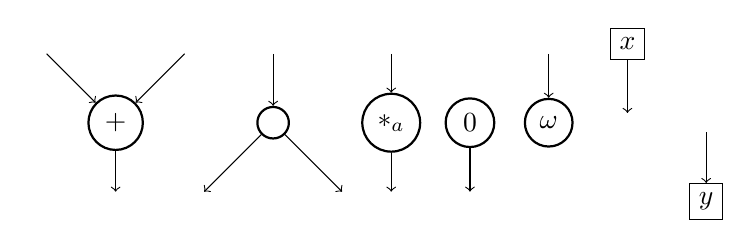
\begin{tikzpicture}
    \tikzstyle{node}=[circle,thick,draw=black,minimum size=4mm]
    \tikzstyle{arg}=[rectangle,thin,draw=black,minimum size=4mm]
    
    \begin{scope}
      \node(in1){};
      \node(nop)[right of=in1]{};
      \node(in2)[right of=nop]{};

      \node[node](plus)[below of=nop]{$+$};
      \node(out)[below of=plus]{};

      \path[->]
      (in1) edge (plus)
      (in2) edge (plus)
      (plus) edge (out);
    \end{scope}
    
    \begin{scope}[xshift=30mm]
      \node(in){};
      \node[node](hub)[below of=in]{$\hub$};
      \node(nop)[below of=hub]{};
      \node(out1)[left of=nop]{};
      \node(out2)[right of=nop]{};

      \path[->]
      (in) edge (hub)
      (hub) edge (out1)
      (hub) edge (out2);
    \end{scope}
    
    \begin{scope}[xshift=45mm]
      \node(in){};
      \node[node](times)[below of=in]{$\rmul{a}$};
      \node(out)[below of=times]{};

      \path[->]
      (in) edge (times)
      (times) edge (out);
    \end{scope}

    \begin{scope}[xshift=55mm]
      \node(nop){};
      \node[node][below of=nop](create){$0$};
      \node(out)[below of=create]{};
      \path[->] (create) edge (out);
    \end{scope}

    \begin{scope}[xshift=65mm]
      \node(in){};
      \node[node][below of=in](destroy){$\omega$};
      \node(nop)[below of=destroy]{};
      \path[->] (in) edge (destroy);
    \end{scope}

    \begin{scope}[xshift=75mm]
      \node[arg](in){$x$};
      \node[below of=in](out){};
      \path[->] (in) edge (out);
    \end{scope}

    \begin{scope}[xshift=85mm]
      \node(nop){};
      \node[below of=nop](in){};
      \node[arg](out)[below of=in]{$y$};
      \path[->] (in) edge (out);
    \end{scope}
  \end{tikzpicture}
  \caption{Nodes over the standard linear basis: round ones are
    evaluation nodes, square ones are input and output nodes.}
\end{figure}


We call \index{port!input~port}\emph{input ports} the elements of $I$
and \index{port!output~port}\emph{output ports} the elements of $O$,
which we denote respectively by
$\inp(v)$\symb[port-in]{$\inp(v)$}{Input ports of a node} and
$\outp(v)$\symb[port-out]{$\outp(v)$}{Output ports of a
  node}. The cardinalities of $I$ and $O$ are called, respectively,
the \index{node!degree}\emph{in-degree} and \emph{out-degree} of $v$.
We call $f$ the \index{node!value}\emph{value} of $v$ and write
$\beta(v)$ for it.

Nodes over the linear basis are pictured in Figure~\ref{fig:nodes}. We
do not explicitly represent the orderings on $\inp(+)$ and
$\outp(\hub)$ because they are not relevant for the linear basis: in
fact, all operators are commutative.

\begin{definition}[Arithmetic circuit]
  Let $\mathcal{B}$ be an $R$-basis. A (linear)
  \index{arithmetic~circuit}\emph{arithmetic circuit} over
  $(R,\mathcal{B})$ is a tuple $C=(V,E,\le,\le_i,\le_o)$ such that
  \begin{enumerate}
  \item $V$ is a finite set of nodes over $(R,\mathcal{B})$;
  \item $<$ is a total order on $V$, $<_i$ is a total order on the
    input nodes in $V$, $<_o$ is a total order on the output nodes in
    $V$;
  \item let $I=\biguplus_{v\in V}\inp(v)$ and $O=\biguplus_{v\in
      V}\outp(v)$, then $E$ is a bijection from $O$ to $I$ such that
    $E(o)=i$ implies that $o\in\outp(v)$, $i\in\inp(v')$ and $v\lneq
    v'$.
  \end{enumerate}
\end{definition}

In practice, the definition says that $C$ is a directed acyclic
multigraph (also called \index{multiDAG}\emph{multiDAG}), where $V$
are the \index{vertex}vertices, $E$ the \index{edge}edges, and where
the \index{node!degree}degrees of each vertex are prescribed by the
arities of the underlying arithmetic node. Moreover, we add an
ordering on input nodes (vertices of in-degree $0$) and on output
nodes (vertices of out-degree $0$). 

In what follows, we shall call $(V,E)$ the
\index{underlying~graph}\emph{underlying graph} of $C$, and use
classic graph theoretic terms to refer to its properties. We shall
often implicitly make this identification. Thus, we shall represent
$E$ as a set of edges $(o,i)$, and make use of the classic concepts of
\emph{incident} edge, nodes \emph{connected} by an edge,
\index{path}\emph{paths}, etc.

Figure~\ref{fig:circuit} shows two examples of arithmetic circuits.
Input and output nodes are ordered from left to right; ports are not
ordered because the basis is commutative.


\begin{figure}[!ht] \centering
  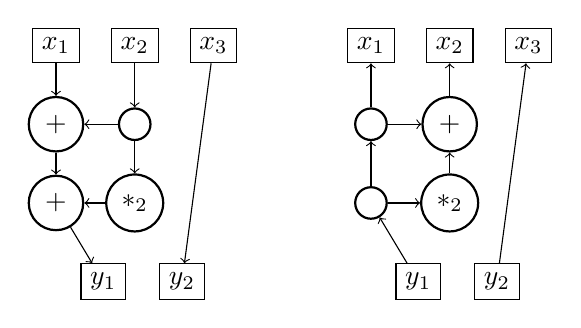
\begin{tikzpicture}
\tikzstyle{node}=[circle,thick,draw=black,minimum size=4mm]
\tikzstyle{arg}=[rectangle,thin,draw=black,minimum size=4mm]
    
    \begin{scope} \node[arg](in1){$x_1$}; \node[arg,right
of=in1](in2){$x_2$}; \node[arg,right of=in2](in3){$x_3$};
      
      \node[node,below of=in1](plus1){$+$}; \node[node,right
of=plus1](H){$\hub$};

      \node[node,below of=plus1](plus2){$+$}; \node[node,right
of=plus2](times){$\rmul{2}$};

      \node[arg,below of=plus2,xshift=6mm](out1){$y_1$};
\node[arg,right of=out1](out2){$y_2$};

      \path[->] (in1) edge (plus1) (in2) edge (H) (in3) edge (out2)
(H) edge (plus1) (H) edge (times) (plus1) edge (plus2) (times) edge
(plus2) (plus2) edge (out1);
    \end{scope}

    \begin{scope}[xshift=4cm]
      \node[arg](in1){$\dual{x_1}$};
      \node[arg,right of=in1](in2){$\dual{x_2}$};
      \node[arg,right of=in2](in3){$\dual{x_3}$};
      
      \node[node,below of=in1](plus1){$\hub$};
      \node[node,right of=plus1](H){$+$};

      \node[node,below of=plus1](plus2){$\hub$};
      \node[node,right of=plus2](times){$\rmul{2}$};

      \node[arg,below of=plus2,xshift=6mm](out1){$\dual{y_1}$};
      \node[arg,right of=out1](out2){$\dual{y_2}$};

      \path[<-]
      (in1) edge (plus1)
      (in2) edge (H)
      (in3) edge (out2)
      (H) edge (plus1)
      (H) edge (times) 
      (plus1) edge (plus2)
      (times) edge (plus2)
      (plus2) edge (out1);
    \end{scope}
  \end{tikzpicture}
  \caption{Two arithmetic circuits over $\Tbasis$. The linear map
    $y_1=x_1+3x_2, y_2=x_3$ is computed by the circuit on the left and
    its dual is computed by the circuit on the right.}
  \label{fig:circuit}
\end{figure}

\begin{definition}[Size, depth]
  \label{def:size}
  Let $C$ be a circuit over $(R,\mathcal{B})$. The
  \index{arithmetic~circuit!size}\emph{size} of $C$, denoted by
  $\size(C)$\symb[circuit-size]{$\size_X(C)$}{Size
    ($X$-weighted) of an arithmetic circuit} is the number of
  evaluation nodes in $V$; the
  \index{arithmetic~circuit!depth}\emph{depth} of $C$, denoted by
  $\depth(C)$\symb[circuit-depth]{$\depth(C)$}{Depth of an
    arithmetic circuit} is the length of the longest directed path
  --in a graph-theoretic sense-- in $(V,E)$.

  Sometimes it is useful to only count certain nodes. Let
  $X\subset\mathcal{B}$, the
  \index{arithmetic~circuit!weighted~size}$X$-weighted size of $C$,
  denoted by $\size_X(C)$ is the number of nodes $v\in V$ such that
  $\beta(v)\in X$.
\end{definition}


\subsection{Semantic of a circuit}
\label{sec:semantic-circuit}
Circuits would be meaningless if they had no semantic attached to
them. Intuitively the semantic corresponds to recursively feed inputs
to the nodes, evaluate $\beta(v)$ at the inputs and collect the
outputs.

\begin{definition}[Evaluation of an arithmetic circuit]
  \label{def:eval}
  \index{arithmetic~circuit!semantic}\index{arithmetic~circuit!evaluation}
  Let $C$ be an arithmetic circuit with $i$ inputs and $o$ outputs,
  then its evaluation is a morphism $\eval_C:R^i\ra
  R^o$\symb[eval]{$\eval_C$}{Evaluation of an arithmetic
    circuit}.

  In order to define it, we simultaneously define the evaluation
  $\eval_v$ of each $v\in V$ and the evaluation $\eval_e$ of each
  $e\in E$. We will denote by $<_v$ the orders on the input and the
  output ports of $v$.
  \begin{itemize}
  \item Let $v\in V$ have out-degree $n$, let its evaluation be
    $\eval_v:R^i\ra R^n$ and let $\pi_1,\ldots,\pi_n$ be the canonical
    projections from $R^n$ to $R$. Let $o_1<_v\cdots<_vo_n$ be the
    output ports of $v$ and let $e_j=\bigl(o_j,E(o_j)\bigr)$ be the
    corresponding edges stemming from $v$, then $\eval_{e_j} =
    \pi_j\circ\eval_v$ for any $j$.
  \item Let $x_1<_i\cdots<_ix_i$ be the input nodes and let
    $\pi_1,\ldots,\pi_i$ be the canonical projections from $R^i$ to
    $R$, then $\eval_{x_j}=\pi_j$ for any $j$.
  \item For every evaluation node $v$ with in-degree $m$, let
    $i_1<_v\cdots<_vi_m$ be the input ports of $v$ and let
    $e_j=\bigl(E^{-1}(i_j),i_j\bigr)$ be the corresponding edges
    incident to $v$, then
    \begin{equation}
      \label{eq:eval_v}
      \eval_v = \beta(v) \circ (\eval_{e_1}, \cdots,\eval_{e_m})
      \text{.}
    \end{equation}
  \item For every output node $y$, let $e\in E$ be the only edge
    incident to $y$, then $\eval_y=\eval_e$.
  \end{itemize}

  We can finally define $\eval_C:R^i\ra R^o$. Let $y_1<_o\cdots<_oy_o$
  be the output nodes, then
  \begin{equation}
    \label{eq:eval}
    \eval_C = \left(\eval_{y_1}, \cdots,\eval_{y_o}\right)
    \text{.}
  \end{equation}
  We also say that $C$ \emph{computes} $\eval_C$.
\end{definition}

It is immediate to verify that $\eval_C$ is a morphism of left
modules, because we only used compositions and direct sums to define
it. The converse is partially true.

\begin{proposition}
  Any morphism of free finite-dimensional $R$-modules can be computed
  by an arithmetic circuit over $(R,\Tbasis)$.
\end{proposition}
\begin{proof}
  Take the matrix associated to such morphism and create a circuit
  that performs the matrix-vector product.
\end{proof}

This also gives an upper bound of $O(mn)$ on the circuit size of a
linear operator $R^m\ra R^n$.

We now define a way of substituting nodes, first syntactically, then
semantically.

\begin{definition}[Syntactic substitution]
  \label{def:syntax-subst}\index{arithmetic~circuit!substitution}
  Let $C=(V,E,\le,\le_i,\le_o)$ be a circuit over $(R,\mathcal{B})$
  and let $C'=(V',E',\le',\le_i',\le_o')$ be a circuit over
  $(R,\mathcal{B}')$. Let $C'$ have $i$ inputs and $o$ outputs and let
  $v\in V$ have in-degree $i$ and out-degree $o$.

  Let $\mathcal{I}$ and $\mathcal{O}$ be monotone bijections
  respectively from $\inp(v)$ to $\inp(C')$ and from $\outp(C')$ to
  $\outp(v)$. We denote by $C[C'/v]$ the circuit
  $(V'',E'',\le'',\le_i'',\le_o'')$ over
  $(R,\mathcal{B}\cup\mathcal{B}')$ defined as follows:
  \begin{itemize}
  \item $V'' = V\uplus (V' - \inp(C') - \outp(C'))$;
  \item $\le_i''=\le_i$, $\le_o''=\le_o$;
  \item $v'\le v''$ if and only if one of the following conditions hold:
    \begin{itemize}
    \item $v',v''\in V$ and $v'\le v''$;
    \item $v',v''\in V'$ and $v'\le' v''$;
    \item $v'\in V$ and $v''\in V'$ and $v'\le v$;
    \item $v'\in V'$ and $v''\in V$ and $v\le v''$;
    \end{itemize}
  \item $E''(o) = \begin{cases}
      E'(o') & \text{if $E(o)\in\inp(v)$ and $\mathcal{I}(E(o))=v'$ and $\outp(v')=\{o'\}$,}\\
      E(o') & \text{if $E'(o)\in\outp(C')$ and $\mathcal{O}(E'(o))=o'$,}\\
      (E\uplus E')(o) & \text{otherwise.}
    \end{cases}$
  \end{itemize}
\end{definition}

\begin{definition}[Semantic substitution]
  \label{def:sem-subst}\index{arithmetic~circuit!substitution}
  Let $C$ be a circuit over $(R,\mathcal{B}\cup\{f\})$ and let $F$ be
  a circuit over $(R,\mathcal{B})$ such that $\eval_F=f$.

  We denote by $C[F/f]$ the circuit over $(R,\mathcal{B})$ where any
  node $v$ of $C$ such that $\beta(v)=f$ has been syntactically
  substituted by $F$.
\end{definition}

The proof of the following proposition is immediate.

\begin{proposition}
  Under the conditions of the previous definition,
  \[\eval_{C[F/f]} = \eval_C \text{.}\]
\end{proposition}

As a shorthand notation, we will draw octogones to signify that a node
has been syntactically substituted by a circuit, without giving the
actual shape of the substituting circuit. Figure
\ref{fig:substitution} shows an example.

\begin{figure}[!ht]
  \label{fig:substitution}
  \centering
  \begin{tikzpicture}
    \tikzstyle{node}=[circle,thick,draw=black,minimum size=4mm]
    \tikzstyle{arg}=[rectangle,thin,draw=black,minimum size=4mm]
    \tikzstyle{subst}=[regular polygon,regular polygon sides=8,thick,draw=black,minimum size=4mm]
    
    \begin{scope}
      \node[arg](in1){$x_1$};
      \node[arg,right of=in1](in2){$x_2$};
      
      \node[node](H)[below of=in2]{$\hub$};
      \node[subst](F)[left of=H]{$F$};

      \node[arg,below of=F,xshift=-6mm](out1){$y_1$};
      \node[arg,right of=out1](out2){$y_2$};
      \node[arg,right of=out2](out3){$y_3$};

      \path[->]
      (in1) edge (F)
      (in2) edge (H)
      (H) edge[bend left=10] (F)
      (H) edge[bend right=10] (F)
      (F) edge (out1)
      (F) edge (out2)
      (F) edge (out3);
    \end{scope}

  \end{tikzpicture}
  \caption{Arithmetic circuit where a node has been syntactically
    substituted by a circuit $F$ with $3$ inputs and $3$ outputs.}
\end{figure}



\subsection{The transposition theorem}
\label{sec:tellegen}
We are now ready to state and prove the
\index{transposition~theorem}\emph{transposition theorem} for
arithmetic circuits. 

We fix a family $(M_i)_{i\in\N}$ of free left $R$-modules, with
$M_i\isom R^i$. Via the isomorphisms, it is straightforward to extend
the definition of arithmetic circuit so that $\eval_c$ is a morphism
$M_i\ra M_o$.  We also fix a family $(N_i)_{i\in\N}$ of free right
$R$-modules, and a family of non-degenerate bilinear forms
\begin{equation}
  \label{eq:240}
  \left(\braket{}{}_i:N_i\times M_i\ra R\right)_{i\in\N}
  \text{.}
\end{equation}
One can think of $M_n$ being $R^n$, $N_n$ being $\dual{(R^n)}$, and
the bilinear forms being the natural ones.

We define the notion of dual circuit, that intuitively corresponds to
\emph{turn all the arrows around}.

\begin{definition}[Dual arithmetic basis]
  Let $\mathcal{B}$ be an arithmetic basis over $R$. The
  \index{dual~arithmetic~basis}\emph{dual basis} $\dual{\mathcal{B}}$
  (with respect to $\braket{}{}_i$) is the basis over $R^\op$
  \begin{equation}
    \label{eq:241}
    \dual{\mathcal{B}} = \{\dual{f} \,|\, f\in\mathcal{B}\}
    \text{.}
  \end{equation}
\end{definition}

In particular, the dual basis to $(R,\Tbasis)$ is 
\begin{equation}
  \label{eq:tbasis-star}
  \tag{$\dual{\Tbasis}$}
  \begin{gathered}
    \begin{aligned}
      +=\dual{\hub} : \dual{(R\oplus R)} &\ra \dual{R}\text{,}  &  \hub=\dual{+} : \dual{R} &\ra \dual{(R\oplus R)}\text{,}\\
      \bra{a,b} &\mapsto \bra{a}+\bra{b}\text{,}\qquad   &      \bra{a} &\mapsto \bra{a,a}\text{,}\\
    \end{aligned}\\ \\
    \begin{aligned}
      \rmul{a}=\dual{(\rmul{a})} : \dual{R} &\ra \dual{R}\text{,} \\
                                             \bra{b} &\mapsto \bra{b}a\text{,}
    \end{aligned}\\ \\
    \begin{aligned}
      0=\dual{\omega} : \dual{0} &\ra \dual{R}\text{,}\qquad  & \omega=\dual{0} : \dual{R} &\ra \dual{0}\text{,} \\
      \bra{\bom} &\mapsto \bra{0}\text{,} &          \bra{a} &\mapsto \bra{\bom}\text{.}
    \end{aligned}
  \end{gathered}
\end{equation}

\begin{definition}[Dual circuit]
  \label{def:dual}\index{arithmetic~circuit!dual}
  Let $C=(V,E,\le,\le_i,\le_o)$ be a circuit over
  $(R,\mathcal{B})$. For any $v\in V$ define
  \begin{equation}
    \label{eq:244}
    \dual{v} =
    \begin{cases}
    (O,I,\dual{f})          &\text{if $v=(I,O,f)$ with $f\ne\emptyset$,}\\
    (O,\emptyset,\emptyset) &\text{if $v=(\emptyset,O,\emptyset)$,}\\
    (\emptyset,I,\emptyset) &\text{if $v=(I,\emptyset,\emptyset)$.}
    \end{cases}
  \end{equation}

  The dual circuit (with respect to $\braket{}{}_i$) of $C$, denoted
  by $\dual{C}$, is the arithmetic circuit over
  $(R^\op,\dual{\mathcal{B}})$
  \[\dual{C} = (\dual{V}, E^{-1},\le',\le_i',\le_o')\text{,}\]
  where $\dual{V}=\{\dual{v}|v\in V\}$ and the orderings are defined
  as follows:
  \begin{align}
    v \le v' \;&\Leftrightarrow\; \dual{v'} \le' \dual{v}\text{,}\\
    v \le_o v' \;&\Leftrightarrow\; \dual{v} \le_o' \dual{v'}\text{,}\\
    v \le_i v' \;&\Leftrightarrow\; \dual{v} \le_i' \dual{v'}\text{.}
  \end{align}
\end{definition}

In particular, this makes $(\dual{V},E^{-1})$ the reverse graph of
$(V,E)$ in a graph-theoretic sense. Figure \ref{fig:circuit} shows two
circuits that are each other's dual. We can now state the
transposition theorem.

\begin{theorem}[Transposition theorem]
  \label{th:tellegen}\index{transposition~theorem}
  Let $C$ be a circuit that computes a morphism $f$, then $\dual{C}$
  computes the dual morphism $\dual{f}$.
\end{theorem}

\pdfmctwo{I explain why I postponed the "elegant" proof.}  In order to
maintain this chapter at the level of elementary linear algebra, we
give here a quite tedious proof: it amounts, in a hidden way, to write
down the matrices of $f$ and $\dual{f}$ and check that they are the
same. In Appendix~\ref{cha:basic-categ-theory} we will give a
conceptually simpler proof, using category theory.

\begin{definition}[Evaluation of a path]
  \index{path!evaluation}
  Let $x$ and $y$ be nodes of $C$ and let $p=(e_1,\ldots,e_k)$ be a
  path from $x$ to $y$.

  If $k=1$, we define $\eval_p$ as the identity map $R\ra R$. If
  $k>1$, for any $1\le i<k$ let the node
  \[\xymatrix{\cdots\ar[r]^{e_i}&v\ar[r]^{e_{i+1}}&\cdots}\]
  have $n_i$ inputs and $m_i$ outputs, and let $\iota:R\ra R^{n_i}$ be
  the injection corresponding to the position of $e_i$ in $\inp(v)$
  and $\pi:R^{m_i}\ra R$ the projection corresponding to the position
  of $e_{i+1}$ in $\outp(v)$, then we define
  \begin{equation}
    \label{eq:252}
    f_i = \pi\circ\beta(v)\circ\iota
    \text{.}
  \end{equation}

  Finally, we define $\eval_p$ as
  \begin{equation}
    \label{eq:247}
    f_{k-1}\circ\cdots\circ f_1
    \text{.}
  \end{equation}
\end{definition}

\begin{lemma}[The electrical network lemma]
  \label{th:electrical-network}
  \index{electrical~network~lemma}
  Let $C$ be an arithmetic circuit, let $x_1\le_i\cdots\le_ix_n$ be
  its input nodes and $y_1\le_o\cdots\le_oy_m$ its output nodes. 
  We have the following identity
  \begin{equation}
    \label{eq:248}
    \pi_j\circ\eval_C\circ\iota_i =
    \sum_{p\in x_i\leadsto y_j}\eval_p
    \quad\text{for any $1\le i\le n$, $1\le j\le m$,}
  \end{equation}
  where the sum ranges over all the distinct paths from $x_i$ to
  $y_j$.
\end{lemma}
\begin{proof}
  \pdfmctwo{Patched proof, finally it is correct!}
  We start by proving that for any node $v$ and any edge
  $v\overset{e}{\ra}v'$
  \begin{equation}
    \label{eq:250}
    \eval_{e} = \sum_{i=1}^n\sum_{p\in x_i\leadsto v\overset{e}{\ra}v'}\eval_p\circ\pi_i
    \text{,}
  \end{equation}
  where $\pi_i:R^n\ra R$ is the $i$-th projection, and the second sum
  ranges over all the distinct paths from $x_i$ to $v'$ passing
  through $e$. We do this by induction on the length of the longest
  path to $v$.

  If the longest path to $v$ has length $0$, then $v$ is one of the
  input nodes, say $x_i$. Then by \hyperref[def:eval]{definition}
  $\eval_e=\pi_i$, and Eq.~\eqref{eq:250} is verified.

  Then, let $v$ be an evaluation node, let $e_1\le_v\ldots\le_ve_k$ be
  the edges incident to $v$, and let $v_1,\ldots,v_k$ be the
  corresponding nodes. Then, by \hyperref[def:eval]{definition}
  \begin{equation}
    \label{eq:251}
    \eval_{e} = \pi_e\circ\beta(v)\circ(\eval_{e_1},\ldots,\eval_{e_k}) =
    \sum_{j=1}^k \pi_e\circ\beta(v)\circ\iota_j\circ\eval_{e_j}
    \text{,}
  \end{equation}
  where $\pi_e$ is the projection corresponding to the position of $e$
  in $\outp(v)$. By induction, this is equivalent to
  \begin{equation}
    \label{eq:253}
    \sum_{j=1}^k\sum_{i=1}^n\sum_{p\in x_i\leadsto v_j\overset{e_j}{\ra}v} \pi_e\circ\beta(v)\circ\iota_j\circ\eval_p\circ\pi_i =
    \sum_{i=1}^n\sum_{p\in x_i\leadsto v\overset{e}{\ra}v'}\eval_p\circ\pi_i
    \text{,}
  \end{equation}
  where the equality comes from Eq.~\eqref{eq:252}.

  Now, by the \hyperref[def:eval]{definition} of $\eval_C$ we have
  \begin{equation}
    \label{eq:254}
    \pi_j\circ\eval_C = \eval_{y_j} = \sum_{i=1}\sum_{p\in x_i\leadsto y_j}\eval_p\circ\pi_i
    \text{,}
  \end{equation}
  and composing on both sides with $\iota_i$ gives Eq.~\eqref{eq:248}.
\end{proof}


\begin{proof}[Proof of the transposition theorem]
  The proof of the transposition theorem is now straightforward. By linearity
  it is enough to prove that
  \begin{equation}
    \label{eq:242}
    \pi_j\circ\eval_C\circ\iota_i =
    \dual{\left(\pi_i\circ\eval_{\dual{C}}\circ\iota_j \right)}
    \quad\text{for any $1\le i\le n$, $1\le j\le m$,}
  \end{equation}
  but this is evident by Eqs.~\eqref{eq:248},~\eqref{eq:247}
  and~\eqref{eq:252}.
\end{proof}

\begin{corollary}
  \label{th:tellegen-coro}
  A linear function $f:R^n\ra R^m$ and its transpose can be computed
  by arithmetic circuits on $(R,\Tbasis)$ of same sizes and depths. In
  particular if $C$ computes $f$ and $\dual{C}$ computes $\dual{f}$,
  \begin{gather*}
    \size_{\{+\}}(C) = \size_{\{\hub\}}(\dual{C}), \qquad  
    \size_{\{\hub\}}(C) = \size_{\{+\}}(\dual{C}), \\
    \size_{\{*_a\}}(C) = \size_{\{*_a\}}(\dual{C})\quad\text{for any $a\in R$},\\
    \size_{\{0\}}(C) = \size_{\{\omega\}}(\dual{C}), \qquad 
    \size_{\{\omega\}}(C) = \size_{\{0\}}(\dual{C}).
  \end{gather*}
\end{corollary}

\begin{remark}
  \label{rk:tellegen}
  The name ``transposition theorem'' is somehow misleading. In fact,
  the theorem says that if $\eval_C$ is the map $x\mapsto xM$ for some
  matrix $M$, then $\eval_{\dual{C}}$ is the map $y\mapsto My$. If $R$
  is commutative, this is equivalent to transpose $M$, but in the
  non-commutative case this is not true anymore. For this reason, we
  shall always prefer the formulation in terms of bilinear forms
  instead of the one in terms of matrices.

  \pdfmcone{Dropped comment about quantum computing: it is
    more complicated than that (and I did not want to develop it in the
    appendix).}  It is also worth noticing that the transposition
  theorem stays true if instead of a bilinear form we had used a
  sesquilinear form (in this case $\dual{(\rmul{a})}=\rmul{\bar{a}}$).
\end{remark}


\begin{nota}
  The name ``The electrical network lemma'' is ours, but it could well
  have been original. The transposition theorem was first discovered
  in electrical network theory by Bordewijk~\cite{bordewijk57}; he
  only showed the case $R=\C$. Some attribute the discovery to
  Tellegen~\cite{burgisser+clausen-shokrollahi,bostan+lecerf+schost:tellegen},
  Bordweijk's advisor, but this is debated~\cite{djb:tellegen}.

  The first complete algebraic proof, treating the case of an
  arbitrary non-commutative ring, is due to
  Fiduccia~\cite{fiduccia:phd}. There have been many rediscoveries of
  the theorem (see~\cite{djb:tellegen}), but Fiduccia's statement stays
  the most general.

  Canny, Kaltofen and Yagati~\cite{canny+kaltofen+yagati89,Ka2K}
  pointed out that the transposition theorem can be proven as a
  special case of Baur and Strassen's differentiation of
  circuits~\cite{baur+strassen83}. We shall come back to this question
  in Section~\ref{sec:autom-diff}.
\end{nota}


\subsection{Circuit families}
\label{sec:uniformity}

A circuit is limited to compute one specific function with inputs and
outputs of fixed size (in terms of elements of $R$). However complexity
theory is interested in algorithms that compute on inputs of variable
size. This leads to study families of circuits.

\begin{definition}[Circuit family]
  Let $\mathcal{B}$ a basis over $R$ and $\pspace$ a set. A
  \index{circuit~family}\emph{circuit family} over
  $(R,\mathcal{B},\pspace)$ is a family of circuits over
  $(R,\mathcal{B})$ indexed by $\pspace$.  $\pspace$ is called the
  \index{parameter~space}\emph{parameter space} of the family. When
  the mapping from $\pspace$ to the circuits is Turing-computable, the
  family is called \index{circuit~family!uniform}\emph{uniform}.
\end{definition}

Algebraic complexity textbooks usually take $\pspace=\N$ and force
$C_n$ to have $n$ inputs. Our construction is more general and lacks
some of the interesting complexity theoretic properties of circuit
families, but its interest will be clear in the next sections.

\begin{definition}[Size and depth functions]
  Let $\mathcal{C} = (C_j)_{j\in\pspace}$ be a circuit family, we
  define the \index{arithmetic~circuit!size}size and
  \index{arithmetic~circuit!depth}depth function as
  \begin{align*}
    \size^{\mathcal{C}}:\pspace&\ra\N  & \depth^{\mathcal{C}}:\pspace&\ra\N\\
                   j&\mapsto\size(C_j) &    j&\mapsto\depth(C_j)
  \end{align*}
  respectively.

  As in definition \ref{def:size}, for $X\subset\mathcal{B}$ we also
  define
  \begin{align*}
    \size^{\mathcal{C}}_X:\pspace&\ra\N\\
                     j&\mapsto\size_X(C_j)
                     \text{ .}
  \end{align*}
\end{definition}

We are mainly interested in uniform circuit families since they are
equivalent to computable functions, the
\hyperref[th:tellegen]{transposition theorem} easily generalizes to
them. We will not study uniform circuit families more in depth; what
we shall do instead, is directly work on computer programs implicitly
representing circuit families and automatically deduce the transposed
family without actually using the circuit model. More details on
uniform circuit families can be found in~\cite{vollmer}.


% Local Variables:
% mode:flyspell
% ispell-local-dictionary:"american"
% mode:TeX-PDF
% mode:reftex
% TeX-master: "../these"
% End:
%

\section{Multilinearity}
\label{sec:multi}

In this section we develop an extension of the transposition theorem
to the multilinear case.  The subject has already been treated by
Hopcroft and Musinski \cite{hopcroft+musinski73} and Fiduccia
\cite{fiduccia:phd}, this section is a mild generalization of their
methods.

\subsection{Multilinear circuits}
\label{sec:multilinear-circuits}
We shall consider \index{multilinear~circuit}\emph{multilinear
  circuits}, i.e.\ circuits that, besides the operators
of~\ref{eq:tbasis}, also contain binary multiplication nodes. The
definitions of the previous section must be adapted to deal with
operators that are not module morphisms, but this generalization is
straightforward (see also Appendix~\ref{cha:basic-categ-theory} for a
clean way of defining arithmetic circuits that supports both linear
and arbitrary circuits).

Multilinear circuits are constructed using the
\index{standard~multilinear~basis}\emph{standard multilinear basis}
$\Sbasis$
\begin{equation}
  \label{eq:sbasis}
  \tag{$\Sbasis$}
  \begin{aligned}
    + : R\times R &\ra R\text{,}    & * : R\times R &\ra R\text{,} &  \hub : R &\ra R\times R\text{,}\\
        a, b &\mapsto a+b\text{,}   &     a, b &\mapsto ab\text{,} &         a &\mapsto a,a\text{,}\\ \\
    \eta_a : \{\bom\} &\ra R\text{,}     &&& \omega : R &\ra \{\bom\}\text{,} \\
          \bom &\mapsto a\text{,} &&&          a &\mapsto \bom\text{.}
  \end{aligned}
\end{equation}


We are going to define a transformation process that transforms a
circuit over $(R,\Sbasis)$ in a (uniform) circuit family over
$(R,\Tbasis)$; the idea is to make any bilinear multiplication node
linear by \emph{fixing} one of its inputs (see
Figure~\ref{fig:linearization}). We call this process
\emph{linearization}, a special case of it has been used in
\cite{gashkov+gashkov05,sergeev08} to transpose circuits that compute
differentials.

\begin{definition}[Zero edge, null edge]
  Let $C$ be a circuit over $(R,\Sbasis)$, a \emph{zero edge} is any
  edge $e$ in $C$ such that one of the following conditions holds:
  \begin{itemize}
  \item $e$ stems from a node $v$ with $\beta(v)=\eta_0$, such an edge
    is also called a \emph{normal} zero edge;
  \item $e$ stems from a node $v$ with $\beta(v)=+$ and whose incident
    edges are both zero;
  \item $e$ stems from a node $v$ with $\beta(v)=*$ and such that at
    least one of the incident edges of $v$ is zero;
  \item $e$ stems from a node $v$ with $\beta(v)=\hub$ and whose input
    edge is zero.
  \end{itemize}
  A \emph{null edge} is any edge $e$ such that one of the following
  conditions holds:
  \begin{itemize}
  \item $e$ is incident to a node $v$ with $\beta(v)=\omega$, such an
    edge is also called a \emph{normal} null edge;
  \item $e$ is incident to a node $v$ with $\beta(v)=\hub$ and whose
    stemming edges are both null;
  \item $e$ is incident to a node $v$ with $\beta(v)\in\{+,*\}$ such
    that its stemming edge is null.
  \end{itemize}
  An output node whose incident edge is zero is called a \emph{zero
    output}, an input node whose stemming edge is null is called a
  \emph{null input}.  A \emph{normal} circuit is a circuit whose zero
  and null edges are all normal.
\end{definition}

Notice that the evaluation of a zero edge or output is the zero
function, the converse is not true.  There is an obvious normalization
technique that takes a generic circuit and transforms it in a normal
circuit having the same evaluation; clearly, the normalization does
not increase the size and the depth of the circuit (it generally
increases $\size_{\{\eta_0,\omega\}}$, though). When necessary, we
will restrict ourselves to normal circuits.

\begin{definition}[Linearization]
  \index{linearization}
  Let $C=(V,E)$ be a circuit over $(R, \Sbasis)$. Let $0=\{v\in
  V|\beta(v)=\eta_0\}$, a linearization of $C$ is a subset
  $\ell\subset\inp(C)\cup 0$ such that:
  \begin{itemize}
  \item for every $v\in V$ with $\beta(v)=+$ either none of its
    incident edges is reachable from $\ell$, or both are;
  \item for every $v\in V$ with $\beta(v)=*$ at most one of the edges
    incident to $v$ is reachable from $\ell$; if $R$ is
    non-commutative, such edge is always the right (left) edge and the
    linearization is called a
    \index{linearization!left}\index{linearization!right}\emph{left
      (right) linearization}.
  \end{itemize}
  If $\ell=\emptyset$, the linearization is called
  \index{linearization!trivial}\emph{trivial}.

  The elements of $\ell\cap\inp(C)$ and $s = \inp(C) - \ell$ are
  respectively called the \index{linear~input}\emph{linear} and
  \index{scalar~input}\emph{scalar} inputs. An edge reachable from
  $\ell$ is called \index{linear!edge}\emph{linear},
  \index{scalar~edge}\emph{scalar} otherwise.
\end{definition}


\begin{definition}[Linearized circuit, scalar part]
  Let $C=(V,E,\le,\le_i,\le_o)$ be a normal circuit over $(R,\Sbasis)$
  and let $\ell$ be a left (resp. right) linearization; without loss
  of generality, we suppose that all the scalar inputs precede the
  linear inputs in the order $\le_i$ (one can always permute inputs).
  
  Let $n$ be the number of scalars for the linearization $\ell$ and
  let $x_1,\ldots,x_n$ be distinct indeterminates over $R$. The
  \index{linearized~circuit}\emph{linearized circuit}
  \begin{equation*}
    C_\ell=(V_\ell,E_\ell,\le_\ell,\le_{i,\ell},\le_{o,\ell})
  \end{equation*}
  is the circuit over $(R[x_1,\ldots,x_n], \Tbasis)$
  (resp. $(R^\op[x_1,\ldots,x_n],\dual{\Tbasis})$) obtained from $C$
  as follows:
  \begin{itemize}
  \item $E_\ell$ is the subset of $E$ containing the linear edges,
  \item $V_\ell$ are the nodes of $V$ adjacent to $E_\ell$, where
    $\beta(v)$ has incurred the following substitutions:
    \begin{itemize}
    \item $\eta_0$ becomes $0$; $+, \hub, \omega$ are preserved;
    \item if $\beta(v)=*$, let $e$ be the only non-linear edge
      incident to $v$ and let
      $a=\eval_e(x_1,\ldots,x_n,\bullet,\ldots,\bullet)$, then $*$
      becomes $\rmul{a}$;
    \item The orders $\le_\ell,\le_{i,\ell},\le_{o,\ell}$ are the
      restriction to $V$ of the original ones.
    \end{itemize}
  \end{itemize}

  The sets $V-V_\ell$ and $E-E_\ell$ are called the \emph{scalar part}
  of $C$.
\end{definition}

Observe that non-linear edges do not depend on linear inputs, thus the
substitution for $*$ is well defined. The trivial linearization gives
the trivial linear circuit with no nodes, hence, its evaluation is the
trivial map $0\ra0$. Figure \ref{fig:linearization} shows an example
of linearized circuit (in the case $R$ is commutative), we gray out
the scalar part of the circuit.

\begin{figure}[!ht]
  \centering
  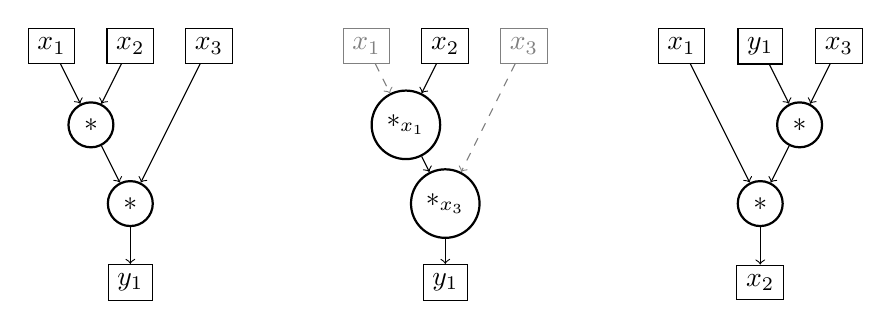
\begin{tikzpicture}
    \tikzstyle{node}=[circle,thick,draw=black,minimum size=4mm]
    \tikzstyle{arg}=[rectangle,thin,draw=black,minimum size=4mm]
    \tikzstyle{nodeg}=[circle,thick,draw=gray,minimum size=4mm]
    \tikzstyle{argg}=[rectangle,thin,draw=gray,minimum size=4mm]
    
    \begin{scope}
      \node[arg](in1){$x_1$};
      \node[arg,right of=in1](in2){$x_2$};
      \node[arg,right of=in2](in3){$x_3$};
      \node[node,below of=in1,xshift=5mm](times1){$*$};
      \node[node,below of=times1,xshift=5mm](times2){$*$};
      \node[arg,below of=times2](out){$y_1$};

      \path[->]
      (in1) edge (times1)
      (in2) edge (times1)
      (times1) edge (times2)
      (in3) edge (times2)
      (times2) edge (out);
    \end{scope}

    \begin{scope}[xshift=4cm]
      \node[argg](in1){\color{gray}{$x_1$}};
      \node[arg,right of=in1](in2){$x_2$};
      \node[argg,right of=in2](in3){\color{gray}{$x_3$}};
      \node[node,below of=in1,xshift=5mm](times1){$\rmul{x_1}$};
      \node[node,below of=times1,xshift=5mm](times2){$\rmul{x_3}$};
      \node[arg,below of=times2](out){$y_1$};

      \path[->]
      (in2) edge (times1)
      (times1) edge (times2)
      (times2) edge (out);
      
      \path[->,draw=gray,dashed]
      (in1) edge (times1)
      (in3) edge (times2);
    \end{scope}

    \begin{scope}[xshift=8cm]
      \node[arg](in1){$x_1$};
      \node[arg,right of=in1](in2){$\dual{y_1}$};
      \node[arg,right of=in2](in3){$x_3$};
      \node[node,below of=in3,xshift=-5mm](times1){$*$};
      \node[node,below of=times1,xshift=-5mm](times2){$*$};
      \node[arg,below of=times2](out){$\dual{x_2}$};

      \path[->]
      (in2) edge (times1)
      (times1) edge (times2)
      (times2) edge (out)
      (in1) edge (times2)
      (in3) edge (times1);
    \end{scope}
  \end{tikzpicture}
  \caption{A circuit over a commutative ring, its linearization for
    $\ell=\{x_2\}$ (scalar edges are grayed out) and its
    $\ell$-dual.}
  \label{fig:linearization}
\end{figure}

Any linearized circuit obviously defines an uniform circuit family
over $(R,\Tbasis)$ (resp. $(R^\op,\dual{\Tbasis})$), thus we can apply
the transposition theorem to the family. But there's more: from a
linearized circuit we can deduce a new circuit over $(R,\Sbasis)$ that
computes the same function as the transposed family.

\begin{definition}[$\ell$-dual]
  \label{def:ell-dual}\index{arithmetic~circuit!l-dual@$\ell$-dual}
  Let $C$ be a normalized circuit over $(R,\Sbasis)$ and let $\ell$ be
  a linearization.  The $\ell$-dual of $C$ is the circuit over
  $(R,\Sbasis)$ obtained by dualizing the linearized circuit $C_\ell$,
  then connecting back the edges of the scalar part to the
  corresponding nodes in $C_\ell$: in doing this nodes with
  $\beta(v)=\rmul{a}$ are changed back to $\beta(v)=*$. The order on
  the nodes of the $\ell$-dual is arbitrary.
\end{definition}

By abuse of notation, the $\ell$-dual will also be noted
$\dual{C_\ell}$. Figure \ref{fig:linearization} shows an example of
$\ell$-dual; notice that $\dual{C_\ell}$ is only defined up to
reordering of the nodes, we will adopt the convention of preserving
the ordering of the linearized circuit, while we take the freedom to
permute the scalar part as it will be more convenient.

\begin{proposition}
  The size of the $\ell$-dual is the same as that of $C$, more
  precisely
  \begin{align*}
    \size_{\{+,\hub\}}(C) &= \size_{\{+,\hub\}}(\dual{C_\ell}), 
    &\size_{\{*\}}(C) &= \size_{\{*\}}(\dual{C_\ell}),\\
    \size_{\{\eta_0,\omega\}}(C) &= \size_{\{\eta_0,\omega\}}(\dual{C_\ell}), 
    &\size_{\{\eta_a|a\ne0\}}(C) &= \size_{\{\eta_a|a\ne0\}}(\dual{C_\ell}).
  \end{align*}
  Its depth is at most twice that of $C$.
\end{proposition}


\subsection{Bilinear chains}
\label{sec:bilinear-chains}

The case of bilinear circuits has received particular interest because
it permits to give lower bounds on the complexity of matrix
multiplication~\cite{fiduccia:phd}. In this section we just point out
how the results of Hopcroft and Musinski~\cite{hopcroft+musinski73}
and Fiduccia~\cite{fiduccia:phd} reduce to ours.

\begin{definition}[Linear chain]
  Let $R$ be non-commutative and let $S\subset R$ be a subring of its
  center. A circuit $C$ over $(R,\Tbasis)$ such that no directed path
  in $C$ contains two nodes $v\ne v'$ with $\beta(v)=\rmul{a}$ and
  $\beta(v')=\rmul{a'}$ where $a,a'\not\in S$ is called an
  \index{linear~chain}\emph{$S$-linear chain}.
\end{definition}

We have seen in Remark~\ref{rk:tellegen} that in the non commutative
case the transposition principle does not \emph{transpose
  matrices}. It is however possible to transpose linear chains.

\begin{definition}[Opposite circuit]
  Let $C=(V,E)$ be a circuit over $(R,\Tbasis)$, the
  \index{arithmetic~circuit!opposite}\emph{opposite circuit} of $C$,
  noted $C^\op$, is the arithmetic circuit over $(R^{\op},\Tbasis)$
  where any $\beta(v)=\rmul{a}$ has been changed to $\rmul{a^\op}$.
\end{definition}

\begin{proposition}
  Let $C$ be a linear chain and let $\eval_C(x)=\trans{x}M$ for some
  matrix $M$, then $\eval_{C^\op}(x)=\trans{M}x$.
\end{proposition}
\begin{proof}
  This is a consequence of the
  \hyperref[th:electrical-network]{electrical network lemma}.  The
  matrix $M$ associated to $\eval_C$ is given by
  \begin{equation}
    \label{eq:243}
    m_{ij} = \pi_j\circ\eval_C\circ\iota_i(1)
    = \sum_{p\in x_i\leadsto y_j}\eval_p(1) =
    \sum_{p\in x_i\leadsto y_j} p_1p_2\cdots p_{n_p}
    \text{,}
  \end{equation}
  where $\rmul{p_1},\ldots,\rmul{p_{n_p}}$ are the scalar
  multiplication nodes on the path $p$.

  Now, by the definition of linear chain, on any path there is at most
  one element not in the center of $R$, thus
  \begin{equation}
    \label{eq:245}
    (p_1p_2\cdots p_{n_p})^\op=p_{1}^\op p_2^\op\cdots p_{n_p}^\op
    \text{,}
  \end{equation}
  and the claim follows.
\end{proof}

Thus, to any linear chain one can associate the four circuits
$C,\dual{C},C^\op,\dual{{C^\op}}$. In~\cite{hopcroft+musinski73,fiduccia:phd},
bilinear chains are considered, i.e.\ bilinear circuits whose only two
non-trivial linearizations are linear chains. The opposite circuit of
a \index{bilinear~chain}bilinear chain is defined by swapping every
multiplication node. Thus, if $C$ is a bilinear chain and
$\ell_1,\ell_2$ its linearizations, one obtains the six circuits
\[C,C^\op,\dual{C_{\ell_1}},\dual{{C_{\ell_1}^\op}},\dual{C_{\ell_2}},\dual{{C_{\ell_2}^\op}}\text{.}\]

Finally, the complexity bounds of~\cite{hopcroft+musinski73}, are
obtained by considering the sets $D=\{\rmul{a}|a\in S\}$ and
$M=\{\rmul{a}|a\not\in S\}$ and realizing that both $\size_D$ and
$\size_M$ are preserved taking the $\ell$-dual and/or the opposite.



% Local Variables:
% mode:flyspell
% ispell-local-dictionary:"american"
% mode:TeX-PDF
% mode:reftex
% TeX-master: "../these"
% End:
%

\section{Automatic differentiation}
\label{sec:autom-diff}

\index{automatic~differentiation}\emph{Automatic differentiation}
(\index{AD@see{automatic~differentiation}}AD) studies the following
question: given a program to evaluate a function $f:R^n\ra R$ at a
point of $R^n$, how much does it cost to evaluate the gradient $\nabla
f$ at a point of $R^n$. More generally, one can consider functions
$R^n\ra R^n$ and ask for the evaluation of the Jacobian matrix $J_f$.

\subsection{From automatic differentiation to transposition}
\label{sec:from-autom-diff}
Transposition of linear straight line programs reduces to automatic
differentiation, in fact, if one has a program computing a linear
function $f:R^n\ra R^m$ and a $\ell\in\dual{(R^m)}$,
\begin{equation}
  \label{eq:261}
  \nabla (\ell\circ f) =
  \left(\frac{\partial \ell\circ f}{\partial x_1},\ldots,\frac{\partial \ell\circ f}{\partial x_n}\right) =
  \left(\braket{\dual{f}(\ell)}{\basis{e}_1},\ldots,\braket{\dual{f}(\ell)}{\basis{e}_n}\right)
  \text{,}
\end{equation}
where $(\basis{e}_1,\ldots,\basis{e}_n)$ is the standard basis of
$R^n$. Thus, differentiating the program for $\ell\circ f$ yields the
coordinates of $\dual{f}(\ell)$ on the standard basis of
$\dual{(R^n)}$ as requested.

Automatic differentiation is widely used in numerical computations and
this is why there is an extensive literature on it. In particular the
\index{reverse~mode}\index{automatic~differentiation!reverse~mode}\emph{reverse
  mode} with the
\index{automatic~differentiation!checkpoint~method}\index{checkpoint~method}\emph{checkpoint
  method} of Griewank~\cite{griewank92} implies that automatic
differentiation of functions $R^n\ra R$ can be done with a constant
factor penalty in algebraic time complexity and an $O(\log(n))$
penalty in algebraic space complexity. However, this is still far from
the bounds of Theorem~\ref{th:tellegen-R-algeb}.

Using the method of the
\index{adjoint~code}\index{automatic~differentiation!adjoint~code}{adjoint
  code} with optimizations for linear
instructions~\cite{gilbert+levey+masse91}, it is possible to save even
more and ultimately reduce to the bounds of the transposition
principle. This is not surprising as the adjoint code on linear
programs is exactly the same thing as the transposition of linear
straight line programs we saw in the previous section.

However, automatic differentiation uses a lot of machinery that has
been tailored for non-linear programs. Using it for transposition is
just overkill. Even worse, it is clumsy because automatic
differentiation is built on top of the transposition principle as it
was pointed out by~\cite{gashkov+gashkov05}. To see this we shall
briefly recall how automatic differentiation works on arithmetic
circuits.

\subsection{Differentiation of arithmetic circuits}
\label{sec:diff-arithm-circ}
\pdfmargincomment{Éric: justement, "arithmetic circuits" implique
  qu'on est dans le monde de la complexité algébrique, non? Il ne me
  semble pas qu'il y ait des travaux précédents à Baur-Strassen qui
  parlent de differentiation ET de circuits arithmétiques.} The first
result on differentiation of arithmetic circuits is due to Baur and
Strassen~\cite{baur+strassen83}. They show that a non-linear
arithmetic circuit that computes a function $f:R^n\ra R$ can be
transformed in a circuit to compute $f$ and $\nabla f$ with a
three-fold increase in size. Gashkov and
Gashkov~\cite{gashkov+gashkov05} interpret their method as a
transformation that yields a circuit to compute $f$ and the
differential $\diff f$ at a point $x$ and $n$ differential inputs
$\diff x_1,\ldots,\diff x_n$; then, an application of the
transposition principle on linearized circuits as in
Section~\ref{sec:multilinear-circuits}, yields the original result of
Baur and Strassen.

Here we describe the transformation of~\cite{gashkov+gashkov05} in a
simplified manner. A complete description can be found
in~\cite{gashkov+gashkov05,sergeev08}.

For simplicity, we consider an arithmetic circuit $C$ over a
non-linear basis $\mathcal{B}$ over $\R$ made exclusively of
everywhere continuously derivable functions (w.r.t the standard metric
of the Euclidean space $\R^n$). We describe a technique to compute the
differential of $\eval_C$ at a point $a\in\R^n$.

\begin{definition}[Differential of a circuit]
  \index{differential~of~a~circuit}\index{arithmetic~circuit!differential}
  Let $C=(V,E,\le,\le_i,\le_o)$ be a circuit over $(\R,\mathcal{B})$
  with $n$ inputs and $m$ outputs and let $a\in\R^n$. For any function
  $f\in\mathcal{B}$, we denote by $J_f$ its Jacobian. 

  The \emph{differential} of $C$ at $a$, denoted by $\diff_a C$, is
  obtained by substituting each $\beta(v)$ with
  \begin{equation}
    \label{eq:derivative}
    \beta'(v)=J_f\left(\eval_{e_1}(a),\ldots,\eval_{e_k}(a)\right)
  \end{equation}
  for any $v\in V$, where $e_1,\ldots,e_k$ are the edges incident to
  $v$.
\end{definition}

\begin{figure}[!ht]
  \centering
  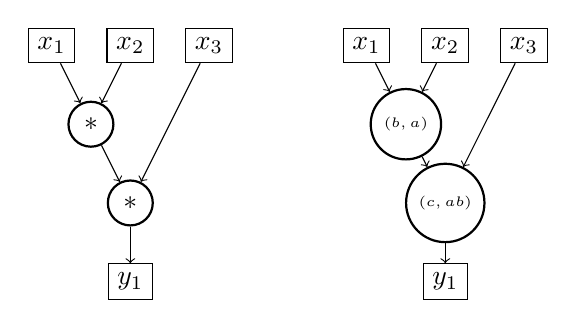
\begin{tikzpicture}
    \tikzstyle{node}=[circle,thick,draw=black,minimum size=4mm]
    \tikzstyle{arg}=[rectangle,thin,draw=black,minimum size=4mm]
    
    \begin{scope}
      \node[arg](in1){$x_1$};
      \node[arg,right of=in1](in2){$x_2$};
      \node[arg,right of=in2](in3){$x_3$};
      \node[node,below of=in1,xshift=5mm](times1){$*$};
      \node[node,below of=times1,xshift=5mm](times2){$*$};
      \node[arg,below of=times2](out){$y_1$};

      \path[->]
      (in1) edge (times1)
      (in2) edge (times1)
      (times1) edge (times2)
      (in3) edge (times2)
      (times2) edge (out);
    \end{scope}

    \begin{scope}[xshift=4cm]
      \node[arg](in1){$\diff x_1$};
      \node[arg,right of=in1](in2){$\diff x_2$};
      \node[arg,right of=in2](in3){$\diff x_3$};
      \node[node,below of=in1,xshift=5mm](times1){\tiny$(b,a)$};
      \node[node,below of=times1,xshift=5mm](times2){\tiny$(c,ab)$};
      \node[arg,below of=times2](out){$\diff y_1$};

      \path[->]
      (in1) edge (times1)
      (in2) edge (times1)
      (times1) edge (times2)
      (in3) edge (times2)
      (times2) edge (out);
    \end{scope}
  \end{tikzpicture}
  \caption{A circuit and its derivative at the point $(a,b,c)$. We
    have replaced multiplication nodes with linear applications
    represented by $1\times2$ matrices.}
  \label{fig:derivative}
\end{figure}


\begin{proposition}
  The differential of a circuit satisfies $\eval_{\diff_aC}=J_{\eval_C}(a)$ for any $a\in\R^n$.
\end{proposition}
\begin{proof}
  Let $e$ be and edge of $C$, we shall denote by $\eval_e$ its
  evaluation as in Definition~\ref{def:eval}, and by $\eval_e'$ the
  evaluation of the corresponding edge in $\diff_a C$.  We prove that
  for any $a\in\R^n$ and for any edge $e$ of $C$, the differential of
  $\eval_e$ at $a$ is $\eval_e'$.  The proof is by induction and
  follows by the chain rule.

  Let $x_1\le_i\cdots\le_ix_n$ be the inputs of $C$, we write
  $f(\lst{x})$ for $f(x_1,\ldots,x_n)$.  Let $v$ be a node, let
  $e_1\le_v\cdots\le_ve_k$ be its input edges and let $e$ be the
  $i$-th output edge. Set $f=\beta(v)$, then by
  \hyperref[def:eval]{definition}
  \begin{equation}
    \label{eq:266}
    \begin{aligned}
      \eval_v &= f \circ (\eval_{e_1},\ldots,\eval_{e_k})\text{,}\\
      \eval_e &= \pi_i\circ\eval_v \text{,}
    \end{aligned}
  \end{equation}
  where $\pi_i$ is the $i$-th projection. Then, the Jacobian matrix of
  $\eval_v$ is
  \begin{equation}
    \label{eq:267}
    J_{\eval_v}(\lst{x}) =
    J_f(\eval_{e_1},\ldots,\eval_{e_k}) J_{(\eval_{e_1},\ldots,\eval_{e_k})} (\lst{x})
    \text{.}
  \end{equation}
  Hence, $\diff_a \eval_v$ is equal to
  \begin{equation}
    \label{eq:268}
    J_{\eval_v}(a)
    \begin{pmatrix}
      \diff_{a} x_1\\\vdots\\\diff_{a} x_n
    \end{pmatrix} =
    \beta'(v)
    \begin{pmatrix}
      \diff_a \eval_{e_1}\\\vdots\\\diff_a \eval_{e_n}
    \end{pmatrix} =
    \beta'(v)\circ (\eval_{e_1}',\ldots,\eval_{e_n}')
    \text{,}
  \end{equation}
  where the last equality follow by induction. By
  \hyperref[def:eval]{definition}, this is the evaluation of $v$ in
  $\diff_{a} C$, and the claim follows by composing with $\pi_i$.
\end{proof}

It is also clear that $\diff_aC$ is defined over a linear basis over
$\R$, thus the \hyperref[th:tellegen]{transposition theorem} applies
to it. In other words we have defined a transformation from circuits
computing derivable functions to linear circuits. 

Also notice that when $C$ is a linear circuit, then simply
$C=\diff_aC$ for any $a$. In this case, Eq.~\eqref{eq:261} amounts to
plug the form $\ell$ at the bottom of $C$, then, transposing
$\diff_aC=C$ and evaluating at $1$ gives the desired coefficients of
$\dual{f}(\ell)$.


\begin{nota}
  The construction of~\cite{gashkov+gashkov05} is more powerful: they
  start from a non-linear circuit $C$ with input nodes
  $x_1,\ldots,x_n$, and they augment it to obtain a non linear circuit
  $C'$ with input nodes $x_1,\ldots,x_n,\diff x_1,\ldots,\diff x_n$;
  this circuit admits a linearization $\ell=\{\diff x_1,\ldots,\diff
  x_n\}$, in the sense of Definition~\ref{def:linearization}, and they
  prove that $C'_\ell=\diff_{\lst{x}} C$. Then, Baur and Strassen's theorem
  follows by considering $\dual{{C'_\ell}}$.
\end{nota}



\subsection{From transposition to automatic differentiation}
\label{sec:from-transp-autom}
The circuit $\diff_a C$ is an important intermediate step to compute
the gradient: any automatic differentiator computes it, either
explicitly or implicitly.

Now $\diff_aC$ can be queried by black-box algorithms to obtain
information about the Jacobian $J_{\eval_C}(a)$. The simplest
application is to compute the directional derivative in $a$ along a
direction $u$: for this task it suffices to evaluate the circuit once,
since $\eval_{\diff_aC}(u)$ is the desired value. Computing the
derivative along $n$ linearly independent directions yields the whole
Jacobian matrix and this roughly corresponds to the
\index{direct~mode}\index{automatic~differentiation!direct~mode}\emph{direct
  mode} in automatic differentiation.

\begin{remark}
  To be more precise, direct mode automatic differentiation constructs
  $\diff_aC$ and evaluates the $n$ directions in parallel, thus
  avoiding the need to store the whole circuit in memory. This is a
  great advantage for iterative code, where $C$ can be represented
  compactly by a for loop, but $\diff_a C$ needs the loop to be
  unrolled.
\end{remark}

When the circuit has many inputs but only one output, there is a more
convenient way to get $\nabla \eval_C$ with only one black-box query:
$\diff_aC$ computes a linear form whose coefficients are exactly the
coefficients of the gradient, thus the dual circuit
$\dual{(\diff_aC)}$ computes the transposed form. The single query
$\eval_{\dual{(\diff_aC)}}(1)$ yields this vector. This is exactly
what is called ``reverse mode'' in automatic differentiation. 

\begin{remark}
  Unlike the direct mode, reverse mode cannot compute
  $\dual{(\diff_aC)}$ and evaluate on a direction in parallel. One
  solution is to store the whole $\diff_aC$ in memory, but this object
  may be too large. The checkpoint method of
  Griewank~\cite{griewank92} computes $\diff_aC$ by \emph{slices} of
  logarithmic size and transposes them one by one. Another way to gain
  space is to observe that the Jacobian linear operations (e.g., sums)
  does not depend on $a$, thus it does not need to be precomputed;
  this technique is suggested in~\cite{gilbert+levey+masse91},
  although it has seldom been implemented.

  Whatever one does to save space, the key observation is the
  following: the generation of code to compute $\diff_a f$ and its
  transposition can be done in two separate phases. Thus, automatic
  differentiation can concentrate of finding techniques to save space
  in the computation of $\diff_a f$, while
  \index{automatic~transposition}\emph{automatic transposition} can
  concentrate on \emph{reversing} code.
\end{remark}

\begin{nota}
  One is not limited to direct or reverse mode: any black-box
  algorithm can be combined with the differential circuit to obtain
  information on the original function. For example Wiedemann's
  algorithm~\cite{wiedemann:sparse} can be used to determine if the
  function is invertible around $x$, and the directional derivatives
  of the inverse can be computed.
\end{nota}




% Local Variables:
% mode:flyspell
% ispell-local-dictionary:"american"
% mode:TeX-PDF
% mode:reftex
% TeX-master: "../these"
% End:
%

\section{Straight Line Programs}
\label{sec:stra-line-progr}

One can view arithmetic circuits as algorithms, where each node is an
elementary step. Then, the size of a circuit is a measure of
complexity in terms of number of elementary (algebraic)
operations. However, arithmetic circuits do not carry any information
about space complexity.

\index{straight~line~program}Straight line programs
(\index{SLP@see{straight~line~program}}SLP) permit to reason about
both space and time complexity: they can be seen as evaluation
strategies for arithmetic circuits, carrying information about
registers to store intermediate results. Informally speaking, they are
programs that are only made of a sequence of assignments (no
branchings, no loops).  See~\cite{burgisser+clausen-shokrollahi} for
formal definitions and proofs.

\pdfmargincomment{More precisions on the algebraic RAM.}
We work in the algebraic \index{RAM~model}RAM model
of~\cite{kaltofen88:gcd}; this is to the classic RAM model what the
BSS model~\cite{BSS} is to the Turing machine. In a slightly
simplified way, an $R$-algebraic RAM (Random Access Machine) has a
memory, made of an infinite set of registers that can contain an
arbitrary element of $R$, and a CPU, that can perform arithmetic
operations on elements of $R$ and store the result in a register.

An SLP can be seen as a program for an algebraic RAM: its inputs are
initially stored in some registers, its instructions are executed in
order, and its outputs are to be read in some other registers. For
example, the program
\begin{equation}
  \label{eq:275}
  \begin{aligned}
    R_3 &\la R_1 + R_2\\
    R_3 &\la R_3 * 3\\
    R_2 &\la R_2 * R_3
  \end{aligned}
\end{equation}
expects is inputs in the registers $R_1$ and $R_2$, performs an
addition, a scalar multiplication and a multiplication, and stores its
output in the registers $R_2$ and $R_3$ (in our context, it is somehow
arbitrary to decide which are the input and output registers). In this
model, the time complexity of a SLP is given by the number of
instructions, the space complexity by the number of different
registers used.



\subsection{The BLS model}
\label{sec:bls-model}
In this section we study a particular family of \emph{linear straight
  line programs} introduced by Bostan, Lecerf and
Schost~\cite{bostan+lecerf+schost:tellegen} to study the transposition
principle. They consider straight line programs consisting uniquely of
the two operations
\begin{align}
  \label{eq:269}
  R_i &\la R_i + R_j
  \text{,}
  &\text{also written }
  R_i \overset{+}{\la} R_j
  \text{,}\\
  \label{eq:272}
  R_i &\la R_i * a
  \text{,}
  &\text{also written }
  R_i \overset{*}{\la} a
  \text{,}
\end{align}
where $R_i,R_j$ are registers and $a\in R$. 

\pdfmargincomment{Slightly rephrased.}
Such SLP's can compute the same morphisms as linear circuits
over the basis $\mathsf{BLS}$:
\begin{equation}
  \tag{$\mathsf{BLS}$}
  \label{eq:246}
  \mathsf{XOR}_1 :
  \begin{pmatrix}
    1 & 0\\1 & 1
  \end{pmatrix}
  \text{,}\quad
  \mathsf{XOR}_2 :
  \begin{pmatrix}
    1 & 1\\0 & 1
  \end{pmatrix}
  \text{,}\quad
  \rmul{a} :
  \begin{pmatrix}
    a
  \end{pmatrix}
  \text{ for $a\in R$.}
\end{equation}
In fact, consider a circuit $C$ over $(R,\mathsf{BLS})$ and let
$x_1,\ldots,x_n$ be its inputs. Allocate $n$ registers
$R_1,\ldots,R_n$ and initialize them to the values of
$x_1,\ldots,x_n$. Then, walk through $C$ in any topological order and
for any $\rmul{a}$ acting on $R_i$ issue the instruction
\begin{equation}
  \label{eq:249}
  R_i \lat a
  \text{,}
\end{equation}
for any $\mathsf{XOR}_1$ acting on $R_i$ and $R_j$ issue the
instruction
\begin{equation}
  \label{eq:255}
  R_i \lap R_j
  \text{,}
\end{equation}
and for any $\mathsf{XOR}_2$ acting on $R_i$ and $R_j$ issue the
instruction
\begin{equation}
  \label{eq:256}
  R_j \lap R_i
  \text{.}
\end{equation}
Observe that all the operators in \ref{eq:246} have the same input and
output arities, then circuits over \ref{eq:246} necessarily have the
same number of inputs and outputs. Hence, if a circuit has $n$ inputs
(and outputs), any topological order yields a straight line program
using $n$ registers by this evaluation strategy.  Inversely, it is
clear that any straight line program using only
instructions~\eqref{eq:269} and~\eqref{eq:272} can be represented by a
circuit over \ref{eq:246} having $n$ inputs (and outputs).

\pdfmargincomment{Added precision on the one-to-many correspondence.}  Thus,
we identify circuits over~\ref{eq:246} with such SLP's (note that the
identification is not one-to-one as different topological orders yield
different SLP's), and define the space complexity in the algebraic RAM
model of a circuit over~\ref{eq:246} as its number of inputs (and
outputs).

Finally, observing that $\mathsf{XOR}_1$ is the dual of
$\mathsf{XOR}_2$, we deduce that any circuit $C$ on $(R,\mathsf{BLS})$
has a dual circuit with the same space and time complexities in the
algebraic RAM model.


\begin{remark}
  Let $(L_1,\ldots,L_k)$ be a SLP on $n$ registers, where $L_i$ is one
  of the instructions~\eqref{eq:269} or~\eqref{eq:272}. By what we
  just said we can take as its dual the sequence
  $(\dual{L_k},\ldots,\dual{L_1})$, where $\dual{L_i}$ is defined as
  \begin{align}
    \label{eq:273}
    \dual{(R_i\overset{+}{\la}R_j)} &= R_j\overset{+}{\la}R_i\text{,}\\
    \dual{(R_i\overset{*}{\la}a)} &= R_i\overset{*}{\la}a\text{.}
  \end{align}
\end{remark}


\subsection{Linear straight line programs}
\label{sec:gener-stra-line}
\pdfmargincomment{"generic" -> "classic"}
The step from the SLP's we just defined to classic linear SLP's is
very small. In fact, all one has to do is simulate the instructions
\begin{align}
  \label{eq:257}
  R_i &\la R_j*a\quad\text{with $i\ne j$,}\\
  \label{eq:258}
  R_i &\la R_j + R_k\quad\text{with $i\ne j,k$.}
\end{align}
The first one can be simulated by the sequence
\begin{equation}
  \label{eq:259}
  \begin{aligned}
    R_i &\lat 0\text{,}\\
    R_i &\lap R_j\text{,}\\
    R_i &\lat a\text{;}
  \end{aligned}
\end{equation}
and the second one by
\begin{equation}
  \label{eq:260}
  \begin{aligned}
    R_i &\lat 0\text{,}\\
    R_i &\lap R_j\text{,}\\
    R_i &\lap R_k\text{.}
  \end{aligned}
\end{equation}
It is reasonable not to count multiplications by $0$, as these just
require to free some memory, than one sees that transposing linear
SLP's preserves the space complexity and loses a factor of at most two
on time complexity. However this is clumsy: one can do much better by
transposing directly the instructions~\eqref{eq:257}
and~\eqref{eq:258}.

\begin{definition}[Double use]
  We say that a register $R_i$ is \index{double~use}\emph{doubly used}
  in a sequence of instructions $(L_1,\ldots,L_n)$ if it appears on
  the right hand side of two instructions $L_i$ and $L_j$, and no
  instruction $L_k$ for $i<k<j$ is of the form~\eqref{eq:257}
  or~\eqref{eq:258}.
\end{definition}

The matrix of the instruction $R_i\la R_j*a$ is
$\left(\begin{smallmatrix}1&0\\a&0\end{smallmatrix}\right)$ in
general, but simply
$\left(\begin{smallmatrix}0&0\\a&0\end{smallmatrix}\right)$ if $R_j$
is not doubly used; in the second case, the transposition is
\begin{equation}
  \label{eq:262}
  \begin{aligned}
    R_j&\la R_i*a\text{,}\\
    R_i&\lat 0\text{.}
  \end{aligned}
\end{equation}
Similarly, the matrix of $R_i\la R_j+R_k$ is 
\begin{equation}
  \label{eq:265}
  \begin{pmatrix}
    0 & 0 & 0\\
    0 & 0 & 0\\
    1 & 1 & 0
  \end{pmatrix}
\end{equation}
if $R_j$ and $R_k$ are not doubly used; this transposes to
\begin{equation}
  \label{eq:263}
  \begin{aligned}
    R_j &\la R_i\text{,}\\
    R_k &\la R_i\text{,}\\
    R_i &\lat 0
  \end{aligned}
\end{equation}
(notice that a double use is introduced by this transposition).

\pdfmargincomment{Removed undefined "self-increment".}
By comparing this to equations~\eqref{eq:259} and~\eqref{eq:260}, one
sees that each double use of a register introduces a
$\overset{+}{\la}$ in the transposed code, and each addition
introduces a double use in the transposed code. This corresponds well
to the duality between $+$ and $\hub$.

In conclusion, one sees that the sum of additions and double uses
stays unchanged when transposing generic straight line
programs. Again, it is reasonable not to count multiplications by $0$
(in fact, they can be merged to the next assignment to the register).
Copies of registers like in~\eqref{eq:263} are still a problem in the
algebraic RAM model, but at a higher level of abstraction they can be
handled using references (or one can simplify the code by hand, if his
code has to run on an algebraic CPU!). Thus we can state the following
version of the transposition theorem for straight line programs.

\begin{theorem}[Transposition theorem]
  \label{th:tellegen-slp}\index{transposition~theorem}
  Any linear straight line program $S$ computing a function $f$ can be
  transformed in a new straight line program $\dual{S}$ computing
  $\dual{f}$.  $S$ and $\dual{S}$ use the same number of
  registers. The sum of the algebraic time complexity and the number
  of double uses of registers is the same for $S$ and $\dual{S}$.
\end{theorem}



\subsection{\texorpdfstring{$R$}{R}-algebraic transforms}
\label{sec:r-algebraic-transforms}
One rarely programs with straight line programs: to make transposition
really useful, we must transpose families of SLP's. Bostan, Lecerf and
Schost consider SLP's parameterized by integers and booleans.

\begin{definition}[algebraic transform]
  \label{def:algebraic-transform}
  Let $R$ be a ring, an \index{algebraic~transform}\emph{$R$-algebraic
    transform} is a program in the algebraic RAM model composed by the
  following constructs:
  \begin{itemize}
  \item linear algebraic assignments of the
    forms~\eqref{eq:269},~\eqref{eq:272},~\eqref{eq:257},~\eqref{eq:258};
  \item for loops with iterator ranging over a list of non-algebraic
    registers;
  \item conditionals with tests over non-algebraic registers;
  \item function calls, recursive function calls.
  \end{itemize}
  If the program is recursive, it must terminate on any valid input.
\end{definition}

By extension, we shall also call $R$-algebraic transform any algorithm
that can be expressed in this model. This is equivalent to consider
circuit families; for example, Algorithm~\ref{alg:r-algeb} corresponds
to a circuit family with parameter space $\N$.


\begin{algorithm}
  \caption{\label{alg:r-algeb}$R$-algebraic algorithm}
  \begin{algorithmic}
    \REQUIRE $a,b\in R$; $n\in\N$.
    \FOR{$i\in[1,\ldots,n]$}
    \IF{$i$ is even}
    \STATE $a \lap b$;
    \ELSE
    \STATE $b \lap a$;
    \ENDIF
    \ENDFOR
    \STATE return $a,b$;
  \end{algorithmic}
\end{algorithm}

 
It is clear that, for any value of the non-algebraic parameters, an
$R$-algebraic transform corresponds to a SLP, then the transposition
theorem can be applied to it. In practice, one leaves conditionals
untouched and reverses for loops; function calls (recursive or not)
are substituted by their transpose. For example,
Algorithm~\ref{alg:r-algeb} becomes Algorithm~\ref{alg:r-algeb-t}.

\begin{algorithm}
  \caption{\label{alg:r-algeb-t}Transposition of
    Algorithm~\ref{alg:r-algeb}}
  \begin{algorithmic}
    \REQUIRE $a,b\in R$; $n\in\N$.
    \FOR{$i\in[n,\ldots,1]$}
    \IF{$i$ is even}
    \STATE $b \lap a$;
    \ELSE
    \STATE $a \lap b$;
    \ENDIF
    \ENDFOR
    \STATE return $a,b$;
  \end{algorithmic}
\end{algorithm}

Putting together the results of this section and the previous ones, we
can now state the transposition theorem for algebraic transforms.

\begin{theorem}[Transposition theorem]
  \label{th:tellegen-R-algeb}\index{transposition~theorem}
  Any $R$-algebraic transform $T$ computing a linear function
  $f$ can be transformed in an $R$-algebraic transform $\dual{T}$
  computing $\dual{f}$.  $T$ and $\dual{T}$ use the same number of
  registers. The sum of the algebraic time complexity and the number
  of double uses of registers is the same for $T$ and $\dual{T}$.
\end{theorem}

\begin{nota}
  Observe that some care must be taken when counting double uses in
  for loops: a single assignment in a for loop counts as $n-1$ double
  uses, where $n$ is the number of times the loop is repeated.
\end{nota}


\subsection{\texorpdfstring{$R$}{R}-algebraic algorithms}
\label{sec:r-algebr-algor}
The transposition theorem for algebraic transforms is an important
result that we shall use in the following chapters. However, if we
want to transpose the multiplication or the Euclidean division of
Section~\ref{sec:transp-algor}, we need to consider SLP's
parameterized by algebraic elements.

With a little of hand waving, the transposition theorem is applied to
algorithms parameterized by algebraic elements
in~\cite{bostan+lecerf+schost:tellegen}:
\begin{quote}
  ``Last, we will consider algorithms mixing linear and non-linear
  precomputations; the transposition principle leaves the latter
  unchanged.''
\end{quote}

We shall call \index{algebraic~algorithm}\emph{$R$-algebraic} any
algorithm that can be expressed in the algebraic RAM model, and that
terminates on any input. Formally, the way an $R$-algebraic algorithm
can be transposed is by \emph{partial
  evaluation}~\cite{consel+danvy93,riazanov+voronkov04,carette+kiselyov+shan09:jfp}.

\begin{definition}[Partial evaluation]
  Let $M,N$ be free $R$-modules (non necessarily finite). Let
  $A:M\times\pspace\ra N$ be an $R$-algebraic algorithm and let $p\in
  \pspace$. The \index{partial~evaluation}\emph{partial evaluation} of
  $A$ on $p$ is the algorithm
  \begin{equation}
    \label{eq:274}
    \begin{aligned}
      A_{p}:L&\ra N\text{,}\\
      x &\mapsto A(x;p)
      \text{.}
    \end{aligned}
  \end{equation}
\end{definition}

If for any $p\in\pspace$ the partial evaluation $A_{p}$ is
a straight line program, then we can apply the transposition theorem
to $A_{p}$. For example, if $M:R[X]\times R[X]\times \N\ra R[X]$ is
a polynomial multiplication algorithm, then for any $b\in R[X]$, the
\emph{transposed multiplication} is $\dual{M_{b,\deg b}}$, as in
Section~\ref{sec:transp-mult}.

There are many strategies to compute partial evaluations, we shall see
one in Section~\ref{sec:texttttransalpyne}. The simplest one is to
evaluate all the expressions that depend on $p$ and store them in
memory so that they can be used in $A_p$ as constants; this is similar
to the linearization of arithmetic circuits we saw in
Section~\ref{sec:multi}. Obviously, the cost in time complexity is
bounded by the time complexity of $A$; however, the cost in space
complexity is also bounded by the time complexity of $A$.

\begin{principle}[Transposition principle]
  \label{th:tellegen-princip}\index{transposition~theorem}\index{transposition~principle}
  Let $\pspace$ be an arbitrary set. Any $R$-algebraic algorithm $A$
  computing a family of linear functions $(f_p:M\ra N)_{p\in\pspace}$
  can be transformed in an $R$-algebraic algorithm $\dual{A}$
  computing the \emph{dual family}
  $(\dual{f}_p:\dual{N}\ra\dual{M})_{p\in\pspace}$. The algebraic time
  and space complexities of $\dual{A}$ are bounded by the time
  complexity of $A$.
\end{principle}

Notice, however, that in many practical instances of transposition,
the partially evaluated values constitute a negligible amount of the
space used by the algorithm. Thus, in practice, transposed algorithms
often have the same space \emph{and} time complexities as the original
ones; this is the case for all the transposed algorithms that appear
in this document.\footnote{Actually, the author is not aware of
  \emph{any} application of the transposition principle where space
  complexity is not preserved, although it is easy to artificially
  create examples that behave badly.}

\begin{nota}
  Is this the end of the story? Probably not. Umans and
  Kedlaya~\cite{kedlaya+umans08} have recently shown an example of
  non-algebraic algorithm that can be transposed with no loss in space
  and time complexity. This makes one wonder what the true limits of
  the transposition principle are.
\end{nota}



%%% Local Variables: 
%%% mode:flyspell
%%% ispell-local-dictionary:"american"
%%% mode: TeX-PDF
%%% mode: reftex
%%% TeX-master: "../these"
%%% End: 


\chapter{Automatic transposition of code}
\section{From circuits to function-level programming}
\label{sec:fp}
\lstset{language=haskell}

In Section \ref{sec:circuits} we saw that the transposition theorem
holds for uniform circuit families.  Informally, an uniform circuit
family can be simulated in a BSS-like model \cite{BSS} such as a
Turing machine with an additional input/output tape where each cell
contains an element of $R$. Then the transposition theorem can be
extended to this context and it is easy to prove that some fundamental
measures such as space and time complexity are preserved by it. This
kind of approach has been used in \cite{BoLeSc03}.

We won't go further in defining a model and proving a transposition
theorem as this is just matter of posing the right definitions and
deriving the (boring) consequences. Here, instead, we are interested
in the real world scenario of transposing a computer program written
in a general purpose programming language. This section studies how an
uniform circuit family can be efficiently simulated in the Haskell
programming language and how its transposition can automatically be
obtained. Nevertheless, this approach has some limitations that we
will address in the next sections.

As we already pointed out in Section \ref{sec:circuits}, evaluation
(and co-evaluation) of arithmetic circuits can be formally defined by
means of a category with finite products (and coproducts). Arithmetic
circuits over $\Tbasis$, in particular, are defined by means of an
\emph{additive category}, that is a category such that $\hom$ sets are
abelian groups, it has \emph{zero morphisms} and it has all finite
\emph{biproducts}.

It can be proven \cite[VIII.2]{McLane} that in an additive category
finite products and coproducts are naturally isomorphic to biproducts.
This is the key argument for the proof of our lemma \ref{th:coeval}
and ultimately leads to the transposition theorem in the special case
of $RMod{R}$.

Modern functional languages too are constructed around the concept of
category: roughly, the types of the language are viewed as objects and
programs as arrows. In this setting, categories are required to be
\emph{Cartesian closed}. This allows to perform \emph{partial
  evaluation} of a function, an operation known as
\emph{currying}. Examples of Cartesian closed categories are
$\mathsf{Set}$ and $\mathsf{Hask}$ --the category of Haskell types--.

Cartesian closed categories cannot be additive, thus it may seem that
our attempts to natively express circuits in functional languages are
doomed. However the Haskell type system is powerful enough to
represent some categories inside it, in particular subcategories of
$\mathsf{Hask}$. It provides a \emph{type class} \lstinline+Category+,
that we reproduce here --following \cite{Yor09}, we use an infix
operator \lstinline+(~>)+ instead of a prefix one as in the standard
Haskell library--.

\begin{lstlisting}
  class Category (~>) => where
    id :: (a ~> a)
    (.) :: (b ~> c) -> (a ~> b) -> (a ~> c)
\end{lstlisting}

In order to behave as a category, an instance of this class shall form
a monoid for the operation \lstinline+(.)+, with \lstinline+id+ being
the identity element. Now this class can be extended to model additive
categories: we first define a class that mimics \emph{Ab-categories},
or \emph{preadditive} categories, that is categories whose $\hom$ sets
are abelian groups.

\begin{lstlisting}
  class Category (~>) => AbCategory (~>) where
    zeroArrow :: (a ~> b)
    (<+>) :: (a ~> b) -> (a ~> b) -> (a ~> b)
\end{lstlisting}
To behave as an Ab-category, an instance shall form an abelian group
for the operation \lstinline|<+>|, with \lstinline+zero+ being the
identity element; it shall also obey a \emph{bilinear law}:
\begin{lstlisting}
  (f <+> g).(h <+> i) = f.h <+> f.i <+> g.h <+> g.i
\end{lstlisting}

Now we give one possible definition of a class that mimics additive
categories.
\begin{lstlisting}
  class AbCategory (~>) => AdditiveCategory (~>) where
    (&&&) :: (a ~> b) -> (a ~> c) -> (a ~> (b, c))
    (|||) :: (a ~> c) -> (b ~> c) -> ((a, b) ~> c)

  first f = f <**> zeroArrow
  second f = zeroArrow <**> f
  left f = f <++> zeroArrow
  right f = zeroArrow <++> f
  f *** g = (first f) ||| (second g)
\end{lstlisting}
For an instance to behave as an additive category it shall satisfy
\begin{lstlisting}
  id *** id = id
  zeroArrow &&& zeroArrow = zeroArrow ||| zeroArrow = zeroArrow
  (f &&& g) <+> (f' &&& g') = (f <+> f') &&& (g <+> g')
  (f ||| g) <+> (f' ||| g') = (f <+> f') ||| (g <+> g')
  (f ||| g) &&& (f' ||| g') = (f &&& f') ||| (g &&& g')
  (f ||| g)  .  (f' &&& g') = f.f' <+> g.g'
\end{lstlisting}

Haskell programmers may have recognized a familiar pattern:
\emph{arrows}. Arrows were introduced in \cite{Hug00} as a
generalization of \emph{monads}, they have been successfully applied
to many different settings such as, for example, solving ordinary
differential equations \cite{LH10}. They are usually understood as
circuits \cite{Pat01}: the standard library class \lstinline+Arrow+ is
roughly equivalent to evaluation of an arithmetic circuit in
$\mathsf{Hask}$ (or $\mathsf{Set}$), while \lstinline+ArrowChoice+ is
roughly equivalent to co-evaluation.

Our \lstinline+AdditiveCategory+ shares similarities with the standard
classes \lstinline+Arrow+, \lstinline+ArrowChoice+,
\lstinline+ArrowZero+ and \lstinline+ArrowPlus+. In particular, it is
equivalent to evaluation of an arithmetic circuit in an additive
category and, by lemma \ref{th:coeval}, to co-evaluation.

An arrow expression is an expression formed uniquely from elementary
arrows and the combinators of \lstinline+AdditiveCategory+. Given an
arrow expression, it is trivial to form its dual: one substitutes
\lstinline|first| with \lstinline|left|, \lstinline|second| with
\lstinline|right|, \lstinline|&&&| with \lstinline&|||& and changes
any \lstinline|f.g| into \lstinline|g.f|. This corresponds to forming
the dual circuit as in definition \ref{def:dual}, thus if
\lstinline+AdditiveCategory+ is instantiated with arrows that
correspond to the elements of the basis\footnote{It is actually enough
  to create the elementary arrows that correspond to $*_a$ for any
  $a\in R$. The combinators \lstinline+&&&+ and \lstinline+|||+
  already imply $+$ and $\hub$.} $\Tbasis$, one obtains the transposed
circuit as in theorem \ref{th:tellegen}. Also notice that Haskell
defines a \lstinline+do+-notation \cite{Pat01} to write down arrow
expressions more conveniently. Dualizing this notation boils down to
applying the transposition algorithm given in Section \ref{todo}.

By writing Haskell functions that return arrows, or, more generally,
functions that have arbitrary types involving arrows, one can express
circuit families and apply the transposition theorem to them by
dualizing each arrow expression appearing in the computation. Figure
\ref{fig:karahask} shows an example of Karatsuba multiplication
written using this technique.

\begin{figure}
  \centering
  
  \caption{The left-linear Karatsuba algorithm.}
  \label{fig:karahask}
\end{figure}


One limitation to this approach is that it cannot be implemented
inside Haskell. As we have defined them, arrows do not remember their
history: the arrow \lstinline+f.g+ is a new arrow that knows nothing
about the pieces that compose it, thus no Haskell function can
transform it in \lstinline+g.f+. There are three solutions to this:
\begin{enumerate}
\item Define \emph{biarrows} instead of arrows \cite{ASWEP05}. This
  way the dual is computed as a side effect of the computation of the
  arrow. The main advantage of this approach is that it is easy to
  implement, its main disadvantage is that it is not compatible with
  the \lstinline+do+ notation, as observed in \cite{ASWEP05}. Another
  minor disadvantage is that the dualization is not transparent as it
  does not happen at the level of the arrow expression, but inside its
  computation.
\item Write a precompiler for Haskell that dualizes arrow
  expressions. The great advantage of this approach is that it permits
  to treat \lstinline+do+-expressions.
\item Implement arrows at the type-level, instead of the function
  level, by defining a type that describes circuits. However this
  approach is not realistic because of its poor efficiency.
\end{enumerate}

A second, fundamental, limitation is that this approach requires the
user to explicitly identify the linear computations by wrapping them
in arrows. This process may be almost as hard as transposing a program
by hand as done by \cite{BoLeSc03} and the resulting code may be
difficult to read (see figure \ref{fig:karahask}). The next Section
studies an alternative approach where the user if freed from the
burden of \emph{linearizing} the program.



% Local Variables:
% mode:flyspell
% ispell-local-dictionary:"american"
% mode:TeX-PDF
% TeX-master: "transAL"
% End:
%

In this chapter we present a joint work with
Schost~\cite{df+schost10}. We study the
\index{automatic~transposition}\emph{automatic transposition} of
generic code (i.e.\ not limited to straight line programs).
Section~\ref{sec:autom-diff} has shown that this has applications in
automatic differentiation, and we will see other applications in the
next chapters.

By looking at a specific subproblem of automatic differentiation, our
goal is to be more efficient and more general. In particular, compared
to the existing implementations of AD tools, we want to:
\begin{itemize}
\item avoid unnecessary space overhead;
\item handle algebraic, rather than just numerical code;
\item handle advanced programming constructs, including recursion and
  algebraic data types;
\item transpose code parameterized by arbitrary algebraic variables.
\end{itemize}

In this chapter we shall abandon the algebraic RAM model we used in
Section~\ref{sec:stra-line-progr} and work on source code
transformation. Implementation details such as knowing what the cost
of copying variables is, shall be ignored: one can assume that a good
compiler will optimize most of these details. Hence, we shall assume
that Theorem~\ref{th:tellegen-R-algeb} really reflects the behavior of
the code we generate.


\section{Inferring linearity}
\label{sec:inference}
\lstset{language=haskell}

By looking at Section~\ref{sec:transp-algor} one sees that often we
want to transpose families of $R$-algebraic algorithms parameterized
by algebraic elements (e.g., we want to transpose the code that for
any $a\in R$ evaluates the map $b\mapsto ab$). This is also necessary
in automatic differentiation, when the code for $\diff_x f$ not only
depends on $\diff x_1,\ldots,\diff x_n$, but also on $x$.

The next section will address the question of how to transpose such
code. This section, instead, asks the question: can a compiler guess
by itself which inputs to a function are parameters, and which are
linear arguments?

The answer is yes. We show how the type system of common statically
typed functional languages can be extended to automatically infer all
the possible \index{linearization}\emph{linearizations} of a computer
program. We first present the non-commutative case, which can be fully
expressed inside the Haskell type system, then we discuss how to
extend to the commutative case.

\paragraph{Linears, scalars}
\label{sec:linears-scalars}
Suppose we have defined some data type \lstinline{R} representing
elements of a ring $R$ together with the usual constants (say
\lstinline{zeroR}, \lstinline{oneR}, etc.), arithmetic operations (say
\lstinline{plus}, \lstinline{times}, etc.), tests and so on. To
simplify, we assume --as usual in algebraic complexity theory-- that
the type \lstinline{R} is isomorphic to $R$, i.e.\ the elements of $R$
can be represented exactly, the operations don't introduce any
rounding error, etc.

For any term involving elements of type \lstinline{R} we would like
the type system to tell us whether its outputs are linear in its
inputs. For example the term
\begin{lstlisting}
  \x y -> plus x y
\end{lstlisting}
has type \lstinline{R -> R -> R}, but we would like the type checker
to also output something like $\ell\ra\ell\ra\ell$ ($\ell$ for
\index{linear~input}\emph{linear}) telling that the term is a
(curryfied) left module homomorphism from $R^2$ to $R$. For
consistency, we want to view constants as mappings from $R^0$ to $R$,
thus for the term \lstinline{zeroR} we want the type checker to
compute something like $0\ra\ell$, that we simply write as $\ell$.

Now, what do we expect about \lstinline{oneR} or \lstinline{times}?
The former is the mapping $\bom\mapsto1$, which is not a module
homomorphism; then, by analogy with
Definition~\ref{def:linearization}, we want the type checker to output
something like $0\ra s$, or simply $s$ ($s$ for
\index{scalar~input}\emph{scalar}). The second can be made into a
linear mapping by \emph{fixing} its second argument (remember that for
the moment we are restricting to left modules) as we did in
Section~\ref{sec:multi}; thus we expect the type checker to output
$\ell\ra s\ra\ell$, meaning that
\begin{lstlisting}
  \x -> times x y
\end{lstlisting}
is a left module homomorphism $R\ra R$ for any \lstinline{y::R}.

Finally consider the following term
\begin{lstlisting}
  z x n = if n <= 0 then zeroR else plus x (z x (n-1))
\end{lstlisting}
as before we expect something like $\ell\ra\N\ra\ell$, meaning that
\begin{lstlisting}
  \x -> z x n
\end{lstlisting}
is a homomorphism $R\ra R$ for any integer \lstinline{n}.

Observe that in order to make a correct inference about a term such as
\begin{lstlisting}
  \x y -> times x (plus y y)
\end{lstlisting}
we must also admit for any of the previous cases the possibility where
everything is a scalar, so that from the hypothesis that
\lstinline{plus} has type $s\ra s\ra s$ we can deduce the correct type
$\ell\ra s\ra\ell$ for the term above. Summarizing, we would like to
have two types \lstinline{L} and \lstinline{S} such that the following
equations hold
\begin{lstlisting}
  plus :: L -> L -> L
  plus :: S -> S -> S
  times :: L -> S -> L
  times :: S -> S -> S
  zeroR :: L
  zeroR :: S
  oneR :: S
\end{lstlisting}

\pdfmargincomment{Better with newtypes, thanks to Mathieu.}
If we define \lstinline{L} and \lstinline{S} as wrappers around
\lstinline{R}
\begin{lstlisting}
  newtype L = Lin R
  newtype S = Sca R
\end{lstlisting}
then, using Haskell type classes
\cite{Walder+Blott-ad-hoc-polymorphism}, we can conveniently express
all the equations above as
\begin{lstlisting}
  class Ring r where
    zero :: r
    (<+>) :: r -> r -> r
    neg :: r -> r
    (<*>) :: r -> S -> r
\end{lstlisting}
together with the obvious \lstinline{instance} definitions (see the
example in Appendix~\ref{cha:line-infer-karats}). 

\pdfmargincomment{Better terminology, thanks to Mathieu.}  For our
inference to work, it is important that \lstinline{L} be an abstract
data type with only the above functions in its interface. On the other
hand, any other function acting on \lstinline{R} can be wrapped inside
a function acting on \lstinline{S} as, for example,
\begin{lstlisting}
  one = Sca oneR
  (Sca a) == (Sca b) = a == b
\end{lstlisting}
or, simply, using a \lstinline{deriving} clause in the declaration of
\lstinline{S}
\begin{lstlisting}
  newtype S = Sca R deriving (Eq)
\end{lstlisting}

If we restrict to terms that do not use the type constructor
\lstinline{Lin}, then we can show that the semantic of a term with
type
\begin{lstlisting}
  L->...->L->L
\end{lstlisting}
is a left module homomorphism.  \pdfmargincomment{More details on the
  simply typed lambda calculus, as suggested by Mathieu.}  The proof
for the full language would be too long, thus we restrict to a simply
typed $\lambda$-calculus with constants. Its terms are defined by the
following grammar
\begin{equation}
  \label{eq:lambda}
  t ::= c \;|\; x \;|\; t_0 t_1 \;|\; \lambda x . t  \text{ ,}
\end{equation}
where $x$ are identifiers and $c$ are constants; its types are
defined by the grammar
\begin{equation}
  \label{eq:77}
  \tau ::= \ell \;|\; s \;|\; \beta \;|\; \tau \ra \tau
  \text{ ,}
\end{equation}
where $\beta$ are the usual base types (integers, booleans, etc.). If
$\Gamma$ is a type environment, by $\Gamma\vdash t::\tau$ we mean that
the term $t$ has type $\tau$ in $\Gamma$.  The semantic of our
calculus is the usual one, based on $\beta\eta$-reduction.

\pdfmargincomment{Careful about lists and tuples, thanks Mathieu!}  We
suppose all the constants above are defined, plus the usual constants
for the other base types; observe that our grammar forbids type
constructors altogether (including \lstinline{Lin} and
\lstinline{Sca}). In this context we use the type names $\ell$ and $s$
in place of the Haskell types \lstinline{L} and \lstinline{S} defined
above. For simplicity, we shall also assume that lists and tuples are
not part of the types of our language; see the end of this section for
a discussion about them.

\begin{definition}[Flipper]
  \pdfmargincomment{Defined the flipper and changed the proof of the
    lemma, thanks to Léo.}  Let $\tau$ be the type
  \begin{equation}
    \label{eq:58}
    \tau = \alpha_0\ra\alpha_1\ra\cdots\ra\alpha_n
  \end{equation}
  with $\alpha_n$ not a function type. Let $I\subset[0,\ldots,n-1]$
  such that $\alpha_i\ne\ell$ if and only if $i\in I$, and let
  $m=\card{I}$.  The \emph{flipper} for $\tau$, denoted by $\flip_\tau$,
  is the term
  \begin{equation}
    \label{eq:60}
    \flip_\tau = \lambda t.\lambda x_{i_1}.\ldots.\lambda x_{i_m}.
    \lambda x_{j_1}.\ldots.\lambda x_{j_{n-m}}.tx_0\cdots x_{n-1}
    \text{,}
  \end{equation}
  with $i_1,\ldots,i_m\in I$ and $j_1,\ldots,j_{n-m}\in\bar{I}$.
\end{definition}

\begin{lemma}
  \label{th:lininference}
  Let $\Gamma\vdash t::\tau$ be a term, let $m,n\ge0$, and let
  $\Gamma\vdash \flip_{\tau}t::\sigma$ with
  \begin{equation}
    \label{eq:264}
    \sigma=\alpha_1\ra\alpha_2\ra\cdots\ra\alpha_m\ra\underbrace{\ell\ra\cdots\ra\ell}_{\text{$n$ times}}\ra\beta
    \text{,}    
  \end{equation}
  with $\alpha_i\ne\ell$ and $\beta$ not a function type. Let
  $\Delta_i\vdash s_i::\alpha_i$ for $1\le i\le m$. The semantic of
  \begin{equation}
    \label{eq:270}
    \Gamma,\Delta_1,\ldots,\Delta_m\vdash \flip_\tau ts_1\cdots s_m
  \end{equation}
  is
  \begin{enumerate}
  \item\label{item:1} a constant function if $\beta\ne\ell$,
  \item\label{item:2} a module homomorphism $R^n\ra R$ if $\beta=\ell$,
  \end{enumerate}
  assuming the free variables in $t,s_1,\ldots,s_m$
  satisfy~\ref{item:1} or~\ref{item:2}.
\end{lemma}
\begin{proof}
  We distinguish the following cases.
  \begin{itemize}
  \item $\Gamma\vdash c$. All the constants satisfy
    either~\ref{item:1} or~\ref{item:2}. We just work out $0$ and $+$
    defined above and leave the others to the reader; in both cases
    $\flip_\tau c=c$ up to $\beta\eta$-conversion.
    \begin{itemize}
    \item $\Gamma\vdash0::\ell$ is the map $\bom\mapsto 0$, thus a
      (constant) morphism.
    \item $\Gamma\vdash0::s$ is the map $\bom\mapsto 0$, thus a constant
      (morphism).
    \item $\Gamma\vdash+::\ell\ra\ell\ra\ell$ is the map $a,b\mapsto
      a+b$. A morphism.
    \item $\Gamma\vdash+::s\ra s\ra s$. Take any $a::s$ and $b::s$, then
      $\Gamma\vdash a+b::s$ is a constant.
    \end{itemize}
  \item $\Gamma,x::\alpha\vdash x::\alpha$. The claim follows because
    $x$ is free.
  \item $\Gamma\vdash t_0t_1::\tau$. This is the only real case
    to prove. We distinguish two cases:
    \begin{itemize}
    \item $\Gamma\vdash t_1::\ell$, then, by induction its semantic is
      a morphism $0\ra R$ (because it is $\beta\eta$-equivalent to
      $\flip_\ell t_1$). 

      Let $\Gamma\vdash \flip_\tau t_0t_1::\sigma$, with $\sigma$ as in
      Eq.~\eqref{eq:264}, and let $\Delta_i\vdash s_i$ for $1\le i\le
      m$ be as in the hypothesis.  Let $\Gamma\vdash t_0::\tau_0$ and
      $\Gamma\vdash\flip_{\tau_0}t_0::\sigma_0$, then by induction
      \begin{equation}
        \label{eq:271}
        \Gamma,\Delta_1,\ldots,\Delta_m\vdash t_0'\eqdef\flip_{\tau_0}t_0s_1,\ldots,s_m
      \end{equation}
      is either a morphism $R^{n+1}\ra R$ or a constant function. In
      the first case $t_0't_1$ is a morphism $R^{n'}\ra R$, in the second
      case it is a constant function; in both cases
      \begin{equation}
        \label{eq:74}
        \flip_\tau(t_0t_1)s_1\cdots s_m\xleftrightarrow{\beta\eta}t_0't_1        
      \end{equation}
      and the claim follows.
    \item $\Gamma\vdash t_1::\alpha$ with $\alpha\ne\ell$. Then the
      claim follows directly by induction on $t_0$ and
      $\beta\eta$-conversion, by choosing $s_1=t_1$.
    \end{itemize}
  \item $\Gamma\vdash \lambda x.t::\alpha_1\ra\alpha_2$. By induction
    $\Gamma,x::\alpha_1\vdash t::\alpha_2$ satisfies~\ref{item:1}
    or~\ref{item:2} (assuming $x$ does). We distinguish two cases
    \begin{itemize}
    \item $\alpha_1\ne\ell$, then
      \begin{equation}
        \label{eq:73}
        \lambda x.\flip_{\alpha_2}t\xleftrightarrow{\beta\eta}\flip_{\alpha_1\ra\alpha_2}(\lambda x.t)
        \text{;}
      \end{equation}
    \item $\alpha_1=\ell$, then
      \begin{equation}
        \label{eq:76}
        \lambda x.\flip_{\alpha_2}ts_1\cdots s_m\xleftrightarrow{\beta\eta}
        \flip_{\alpha_1\ra\alpha_2}(\lambda x.t)s_1\cdots s_m
        \text{.}
      \end{equation}
    \end{itemize}
    In both cases, $\lambda x.t$ satisfies~\ref{item:1}
    or~\ref{item:2} accordingly.
  \end{itemize}
\end{proof}

\begin{proposition}
  Let $t:\tau$ be a closed term, let $n\ge0$ and let
  \begin{equation}
    \tau=\underbrace{\ell\ra\cdots\ra\ell}_{\text{$n$ times}}\ra\beta
    \text{,}    
  \end{equation}
  with $\beta$ not a function type. Then, the semantic of $t$ is
  \begin{enumerate}
  \item a constant function if $\beta\ne\ell$,
  \item a module homomorphism $R^n\ra R$ if $\beta=\ell$.
  \end{enumerate}
\end{proposition}

By the proof, it should be now clear why we forbid the type
constructor \lstinline{Lin}. In fact, introducing a term as
\lstinline{Lin oneR :: L} tricks the proof (the type checker) by
making it believe that the function $\bom\mapsto 1$ is a morphism.


\paragraph{The commutative case}
\label{sec:commutative-case}
In the commutative case we shall add a second multiplication operator
allowing multiplication on the left by a scalar
\begin{lstlisting}
  class Ring r => CommRing r where
    (>*<) :: S -> r -> r 
\end{lstlisting}
but this would force the user to chose between the two operators any
time he multiplies two elements of $R$. To avoid this we need to
overload the operator \lstinline{(<*>)} with both type signatures, a
technique sometimes called \emph{ad-hoc} polymorphism
\cite{strachey00}, but this is not possible in Haskell's type system
since the two types are contradictory.  To make it possible we need to
extend the type inference algorithm: our idea is not new, but it has
been rarely implemented because it is not practical for solving
generic \emph{ad-hoc} polymorphism; it perfectly fits the needs of our
special case, though.

First observe that type classes can be translated to ordinary types of
the Hindley-Milner type system as explained in \cite[$\S
4$]{Walder+Blott-ad-hoc-polymorphism}, thus it suffices to modify the
classic type inference algorithm
\cite{Damas+Milner,Cardelli:Typechecking}. Second, observe that there
is some redundancy between the two signatures of \lstinline{(<*>)} and
that a more concise version is
\begin{lstlisting}
  (<*>) :: Ring r => r -> S -> r
  (<*>) :: S -> L -> L
\end{lstlisting}

A review of the Hindley-Milner algorithm and its implementation can be
found in \cite{Cardelli:Typechecking}. The idea is to first assign
type variables to terms, then solve type equations by unifying them.
In our generalization, instead of handling a single unification, we
keep a list of possible unifications: when a type equation implies
that a certain unification is not acceptable, the unification is
discarded from the list; if the list gets empty the term cannot by
typed and an error is returned, otherwise any unification in the list
is valid and is returned.

In practice, the only term that makes the list of unification grow is
\lstinline{(<*>)}: any time an equation involving it has to be solved,
the list of unifications potentially doubles. This exponential
increase is the reason why this solution is not practical to solve
generic \emph{ad-hoc} polymorphism; but in our case we really are
interested in knowing all the possible types of a term because each of
them gives rise to a different linearization and, hence, to a
different transposition.

\paragraph{Modules}
\label{sec:modules}
Finally we remark that by allowing tuples and lists,
Lemma~\ref{th:lininference} can be generalized to morphisms $R^m\ra
R^n$ and even to infinite dimensional modules using lazy
lists. Elements of type \lstinline{L}, \lstinline{[L]},
\lstinline{(L,L)}, etc. share a common pattern: they can be viewed as
$R$-modules. It is convenient to summarize their properties in an
unique interface\footnote{We make use of some experimental modules of
  Haskell: this codes needs the flags
  \lstinline{-XMultiParamTypeClasses},
  \lstinline{-XFunctionalDependencies} and
  \lstinline{-XFlexibleInstances} in order to work.}
\begin{lstlisting}
  class Ring r => Module m r | m -> r where
    zeroM :: m
    (<<*) :: m -> S -> m
    (>>>) :: m -> Integer -> r
    (<<<) :: r -> Integer -> m
    (<++>) :: m -> m -> m
    add :: m -> m -> Integer -> m
    add a b n = foldl (<++>) zeroM
                [((a>>>i) <+> (b>>>i))<<<i | i <- [1..n]]
\end{lstlisting}

Instances of this class represent free $R$-modules: \lstinline{zeroM}
is the zero element, \lstinline{(<<*)} is scalar multiplication,
\lstinline{(<++>)} is addition, \lstinline{(<<<)} and
\lstinline{(>>>)} are canonical injections and projections.

This interface adds nothing to the linearity inference system, but we
will need it in Section~\ref{sec:texttttransalpyne}.  Also notice the
presence of the operator \lstinline{add} that performs addition up to
a truncation order, it is of no great importance in this section, but
for efficiency reasons we will eventually prefer it to plain addition.

A fully worked Haskell example of the ideas presented in this section
(without the extension to the commutative case) is given in
Appendix~\ref{cha:line-infer-karats} where we implement Karatsuba
multiplication of polynomials in $\Z[X]$.


% Local Variables:
% mode:flyspell
% ispell-local-dictionary:"american"
% mode:TeX-PDF
% mode: reftex
% TeX-master: "../these"
% End:
%

\section{\tAL}
\label{sec:transAL}

In the previous Section we saw how the scalar and linear parts of a
computation can be automatically inferred through type checking, this
is however not enough to generate transposed code for a generic
program. In this section we define \tAL{}, a very narrow sublanguage
of purely functional languages, and give an algorithm to transpose
programs written in it. Our approach is similar to \cite{BoLeSc03},
but \tAL{} is more powerful than the language defined there.

The main obstacle to transposition of $\lambda$-terms is the
possibility to form terms whose types contain an arbitrary number of
arrows; transposition, on the other hand, only deals with types
containing one unique arrow. To avoid this problem \tAL{} only permits
to declare function types with one arrow, it is defined by the
following EBNF grammar
\begin{align}
  S &::= F^\ast\\
  \tau &::= \ell \;|\; s \;|\; \ldots\\
  A &::= x::\tau\\
  \label{eq:tAL-exp}
  E &::= A^\ast\\
  \label{eq:tAL-if}
  E &::= A_b \;?\; E_i : E_e\\
  \label{eq:tAL-apply}
  E &::= f \al A^\ast\\
  \label{eq:tAL-let}
  E &::= A^\ast\la E_1.E_2\\
  \label{eq:tAL-fun}
  F &::= f = \proc A_i^\ast \ra E
\end{align}
where $x$ are identifiers and $f$ function names (the two namespaces
are separate). Its semantics are given by the following translation to
a functional language (using Haskell syntax)
\begin{align}
  [x_1::\tau_1\cdots x_n::\tau_n]_\delta &\quad=_\delta\quad (x_1::\tau_1,\ldots,x_n::\tau_n)
  \quad\text{,}\\
  [A_b \;?\; E_i : E_e]_\delta &\quad=_\delta\quad
  \text{if }A_b\text{ then }[E_i]_\delta\text{ else }[E_e]_\delta
  \quad\text{,}\\
  [f \al A_i^\ast]_\delta &\quad=_\delta\quad
  f [A_i^\ast]_\delta \quad\text{,}\\
  [A^\ast\la E_1.E_2]_\delta &\quad=_\delta\quad
  \text{let } [A^\ast]_\delta = [E_1]_\delta \text{ in } [E_2]_\delta
  \quad\text{,}\\
  [f = \proc A_i^\ast \ra E]_\delta &\quad=_\delta\quad
  f = \lambda [A_i^\ast]_\delta.[E]_\delta\quad\text{.}
\end{align}
For simplicity, we assume a strict evaluation strategy.

Some functions and identifiers are supposed predefined in \tAL{}:
besides the usual arithmetic and logic constants, there are the
constants \lstinline{zero}, \lstinline{(<+>)}, etc., defined in the
previous Section. Constants of function type are exported to \tAL{} as
predefined functions, constants of non-function type as identifiers,
with the only exception of \lstinline{zero} that is exported as a
function of type $()\ra\tau$.

\tAL{} programs must be valid programs after translation to the
functional language and they must type correctly according to the
rules given in the previous Section; in practice the types of
identifiers could be omitted since they can automatically be computed
by the generalized Hindley-Milner inference we sketched there, but we
explicitly list them in \tAL{} for simplicity. In our grammar we only
listed the types $\ell$ and $s$, since they are the only significant
ones for transposition; in our examples we will note $\ast$ for any
type different from $\ell$ and $s$, or simply omit it.

A \tAL{} program is then just a collection of function definitions,
here's an example that multiplies an element $x$ by a scalar $n\in\Z$:
\begin{equation}
  \label{eq:tALprog}
  \begin{aligned}
    &f = \proc x::\ell \;\; n::\ast \ra\\[-1ex]
    &\qquad b::\ast \la (==) \al n::\ast \;\; 0::\ast\\[-1ex]
    &\qquad b::\ast \;?\\[-1ex]
    &\qquad\qquad \text{zero} \al\\[-1ex]
    &\qquad :\\[-1ex]
    &\qquad\qquad n::\ast \la (-) \al n::\ast \;\; 1::\ast.\\[-1ex]
    &\qquad\qquad y::\ell \la f \al x::\ell \;\; n::\ast.\\[-1ex]
    &\qquad\qquad (\langle+\rangle) \al x::\ell \;\; y::\ell\\[-1ex]
  \end{aligned}
\end{equation}

\tAL{} programs are very similar to straight line programs, in fact,
avoiding the production \eqref{eq:tAL-if} and recursive calls, the two
are strictly equivalent. Just like straight line programs are
isomorphic to circuits \cite[Lemma 13.17]{BuClSh}, terminating \tAL{}
programs are isomorphic to circuit families. To prove this, we
\emph{fix} the values of the variables appearing in the tests of
conditional statements, then a \tAL{} function is just a straight line
program. Furthermore, if we also \emph{fix} all the variables of type
$*$, then we obtain circuit families over $(R,\Sbasis)$; if we
\emph{fix} variables of type $s$ too, we obtain families over
$(R,\Tbasis)$.

We only detail the last isomorphism. First we need to distinguish the
scalar and the linear part of the computation.

\begin{definition}[Scalar restriction]
  The \emph{scalar restriction} of a predefined function $f$, noted
  $\s{f}$, is $f$ itself if its type does not involve any $\ell$, the
  zero function $()\mapsto()$ otherwise. 

  The \emph{scalar restriction} of a \tAL{} function $f$ is defined
  together with the \emph{scalar restriction} $\s{t}$ of a \tAL{} term
  $t$ as follows:

  \begin{align}
    \s{x::\ell\;A^\ast} &\quad=\quad \s{A^\ast} \text{ ,}\\
    \s{x::\tau\;A^\ast} &\quad=\quad x::\tau\;\s{A^\ast}
    \qquad\text{if $\tau\ne\ell$,}\\
    \s{A_b\,?\,E_i:E_e} &\quad=\quad A_b\,?\,\s{E_i}:\s{E_e} \text{ ,}\\
    \notag
    \label{eq:scalar-let}
    \s{f \al A^\ast} &\quad=\quad \s{f} \al \s{A^\ast}
    \text{ ,}\\
    \s{A^\ast\la E_1.E_2} &\quad=\quad \s{A_o^\ast}\la\s{E_1}.\s{E_2}\text{ ,}\\
    \label{eq:scalar-fun}
    \s{f = \proc A_i^\ast\ra E} &\quad=\quad \s{f} = \proc \s{A_i^\ast}\ra\s{E}
    \text{ .}
  \end{align}
\end{definition}

In practice, scalar restriction removes all the names having type
$\ell$ from a function definition. Notice that if $t$ is a valid term,
then $\s{t}$ is valid too: it can be easily shown, in fact, that no
identifier with type $\tau\ne\ell$ depends on any identifier with type
$\ell$.

In the following definition we make use of an environment $\Gamma$,
that is a partial function from names to values.  Let $\Gamma$ be an
environment such that it is defined on all the free variables of a
\tAL{} expression $E$, then the evaluation of $E$ in $\Gamma$, noted
$\Gamma(E)$, is obtained by assigning the values in $\Gamma$ to its
free variables and then evaluating as defined by the semantics.  The
environment $\Gamma:A^\ast\la E$ is the environment $\Gamma$ augmented
by matching the names in $A^\ast$ to the value of $\Gamma(E)$.

\begin{definition}[Linearization of predefined functions]
  Let $v$ be a value of type $s$, the \emph{linearization} by $s$ of
  \lstinline{<*>}$::\ell\ra s\ra\ell$, noted \lstinline{<*>}$_v$, is
  the section $($\lstinline{<*>}$v)$; the linearization of
  \lstinline{<*>}$::s\ra\ell\ra\ell$ is also noted\lstinline{<*>}$_v$
  and is defined analogously. Since the type is always specified by
  the context, we never need to precise which of the two
  linearizations we are talking about.
  
  The functions \lstinline{zero}, \lstinline{<+>} and \lstinline{neg}
  are their own linearization if and only if their type contains
  $\ell$'s. The linearization of any other predefined function is the
  zero function $()\mapsto()$.
\end{definition}

\begin{definition}[Linearization]
  Let $f=\proc x_1::\tau_1\cdots x_n::\tau_n\ra E$ be the definition
  of a \tAL{} function. Up to permutation of the indices, we can
  suppose that $\tau_i=\ell$ if and only if $i\le m$. Let $v_i$ be a
  value of type $\tau_i$ for any $m<i\le n$, the \emph{linearization}
  by $(v_i)_i$ of $f$ is the function defined by
  \begin{equation}
    f_{(v_i)_i} = \proc x_1::\tau_1\cdots x_m::\tau_m\ra [E]_\Gamma
    \text{ ,}
  \end{equation}
  where $\Gamma$ is the environment defined by
  \begin{equation}
    \Gamma(x) =
    \begin{cases}
      v_i \quad\text{if $x=x_i$ for some $i\in[m+1,\ldots,n]$,}\\
      \text{undefined otherwise,}
    \end{cases}
  \end{equation}
  and $[E]_\Gamma$ is defined by the following rules:
  \begin{align}
    \l{x::\ell\;A^\ast} &\quad=\quad x::\ell\;\l{A^\ast} \text{ ,}\\
    %%
    \l{x::\tau\;A^\ast} &\quad=\quad \l{A^\ast}
    \qquad\text{if $\tau\ne\ell$,}\\
    %%
    \label{eq:linear-if}
    [x::*\,?\,E_i:E_e]_\Gamma &\quad=\quad 
    [E_i]_\Gamma \qquad\text{if $\Gamma(x)=$ true,}\\
    %%
    \label{eq:linear-else}
    [x::*\,?\,E_i:E_e]_\Gamma &\quad=\quad 
    [E_e]_\Gamma \qquad\text{if $\Gamma(x)=$ false,}\\
    %%
    \label{eq:linear-apply}
    [f \al A^\ast]_\Gamma &\quad=\quad f_{\Gamma(\s{A^\ast})} \al  \l{A^\ast} \text{ ,}\\
    \label{eq:linear-let}
    [A^\ast\la E_1.E_2]_\Gamma &\quad=\quad
    \l{A^\ast}\la[E_1]_\Gamma.[E_2]_{\Gamma:\s{A^\ast}\la\s{E_1}}
    \text{ .}
  \end{align}
\end{definition}

Using the same notation as in the definition, set
$\pspace_f=\prod_{m<i\le n}\tau_i$. Then for any $v\in\pspace_f$,
$f_v$ has no branchings thanks to rules \eqref{eq:linear-if} and
\eqref{eq:linear-else}. If $f$ terminates on some input $u$, then it
terminates for any other input such that its projection on $\pspace_f$
is equal to the projection of $u$, because linear inputs cannot
influence boolean values, thus they cannot influence branchings. This
implies that either $f_v$ terminates on any input or it always
loops.

Suppose that $f_v$ terminates, if we recursively substitute each
expression $g_{v'}\al A^\ast$ with the definition of $g$, then it is
easily seen by induction that this process eventually terminates and
one ends up with a straight-line program over the basis
\lstinline{zero}, \lstinline{<+>}, \lstinline{neg},
\lstinline{<*>}$_a$. Hence $f_v$ is equivalent to an arithmetic
circuit. To summarize, the mapping $v\mapsto f_v$ from $\pspace_f$ to
\tAL{} programs defines an uniform circuit family if and only if $f$
terminates on any input. Here's the linearization of the example
program \eqref{eq:tALprog}

\begin{align}
  &\begin{aligned}
    &f_0 = \proc x::\ell \ra {\tt zero}\al
  \end{aligned}\\[0.5ex]
  &\begin{aligned}
    &f_{n>0} = \proc x::\ell \ra\\[-1ex]
    &\qquad y::\ell \la f_{n-1} \al x::\ell.\\[-1ex]
    &\qquad (\langle+\rangle) \al x::\ell \;\; y::\ell\\[-1ex]
  \end{aligned}
\end{align}


Once a function has been linearized, it is straightforward to write
down its dual: one simply reads it from top to bottom and swaps input
and output arguments to functions as in \cite{BoLeSc03}. The exact
transformation is made slightly technical by rule \eqref{eq:tAL-let};
instead of presenting it we will rather discuss in the next sections
how we practically transpose code in our implementation.

Before discussing practice, we make some remarks on our linearization
technique. First observe that in order to derive a linearization, rule
\eqref{eq:linear-let} forces to evaluate the scalar part first. The
simplest way to achieve this is to evaluate $\s{f} v$ and to store all
the pairs name-value before computing $f_v$. This technique is similar
to what is called \emph{forward sweep} in automatic differentiation
\cite{GVM91,Gri92} and it may seem that its cost is at most a constant
factor of the cost of evaluating the whole $f$, with an additional
penalty in space because all the values of the scalar part must be
hold in memory. There are, however, some important differences:
\begin{itemize}
\item The \emph{forward sweep} is only needed on the scalar part,
  while in automatic differentiation one needs to evaluate the whole
  $f$ before differentiating. In many practical cases, as in our
  example, the scalar part is negligible compared to the rest.
\item In presence of recursive calls, the forward sweep breaks head
  recursion optimization (this is the case in our example). Dually, it
  breaks tail recursion optimization in the transposed function.
\item The use of recursion may make the forward sweep far more
  expensive than just a constant factor. Consider the function
  \begin{equation}
    \begin{aligned}
      &f = \proc c::\ell \;\; d::s \ra\\[-1ex]
      &\qquad b::* \la (>) \al d::s \;\; \text{\tt zero}::s.\\[-1ex]
      &\qquad b::*\;?\\[-1ex]
      &\qquad\qquad t::s \la (\langle-\rangle) \al d::s \;\; \text{\tt one}::s.\\[-1ex]
      &\qquad\qquad x::\ell \;\; y::s \la f \al c::\ell \;\; t::s.\\[-1ex]
      &\qquad\qquad a::\ell \la (\langle*\rangle) \al x::\ell \;\; y::s.\\[-1ex]
      &\qquad\qquad b::s \la (\langle+\rangle) \al y::s\;\;\text{\tt one}::s.\\[-1ex]
      &\qquad\qquad a::\ell\;\;b::s\\[-1ex]
      &\qquad :\\[-1ex]
      &\qquad\qquad c::\ell\;\;d::s
    \end{aligned}
  \end{equation}
  Its linearization is 
  \begin{align}
    &f_0 = \proc c::\ell \ra  c::\ell\\[0.5ex]
    \label{eq:mechant-lin}
    &\begin{aligned}
      &f_d = \proc c::\ell \ra\\[-1ex]
      &\qquad x::\ell \la f_{d-1} \al c::\ell.\\[-1ex]
      &\qquad a::\ell \la (\langle*\rangle)_{\s{f}(d-1)} \al x::\ell.\\[-1ex]
      &\qquad a::\ell\\[-1ex]
    \end{aligned}
  \end{align}
  and its scalar restriction is
  \begin{equation}
    \begin{aligned}
      &\s{f} = \proc d::s \ra\\[-1ex]
      &\qquad b::* \la (>) \al d::s \;\; \text{\tt zero}::s.\\[-1ex]
      &\qquad b::*\;?\\[-1ex]
      &\qquad\qquad t::s \la (\langle-\rangle) \al d::s \;\; \text{\tt one}::s.\\[-1ex]
      &\qquad\qquad y::s \la \s{f} \al t::s.\\[-1ex]
      &\qquad\qquad b::s \la (\langle+\rangle) \al y::s\;\;\text{\tt one}::s.\\[-1ex]
      &\qquad\qquad b::s\\[-1ex]
      &\qquad :\\[-1ex]
      &\qquad\qquad d::s
    \end{aligned}
  \end{equation}
  Thus, in order to compute $f_d$ one has to compute $\s{f}(d-1)$ in
  the forward sweep, and that requires a recursive call to
  $\s{f}(d-2)$. Then one has to compute $f_{d-1}$ and the value of
  $\s{f}(d-2)$ is needed again for this. In conclusion, any recursive
  call is potentially doubled and this can make the overall cost of
  evaluating $f_v$ (or its transpose) much worse than the cost of
  evaluating $f$. The workaround is to realize that all the recursive
  calls to $\s{f}$ always happen with the same arguments, thus it is
  enough to apply a lazy evaluation strategy on the scalar parts by
  memoizing them.
\end{itemize}
Applying all these ideas, we can guarantee that the
linearization/transposition only yields a constant increase in time
and an increase in space that is at most the size of the scalar part

Finally, we remark that \tAL{} is a very limited language as it
doesn't even have support for lists. Functions that act on lists are
usually written using pattern-matching, but this interacts very poorly
with transpostion because the information on which pattern matches the
output is lost. A good compromise is to add two types $M(\ell)$ and
$M(s)$ representing infinite dimensional modules over $R$ and to
expose an interface as in the previous Section. However, this adds
some issues that will be discussed in the next section.


% Local Variables:
% mode:flyspell
% ispell-local-dictionary:"american"
% mode:TeX-PDF
% TeX-master: "transAL"
% End:
%

\chapter{Linearity inference of karatsuba multiplication}
\label{cha:line-infer-karats}

\lstset{language=haskell}

We show here an example of inference of linearity in Haskell, using
the technique described in Section~\ref{sec:inference}. We define type
classes \lstinline{Ring} and \lstinline{Module} to represent
left-linear operations on rings and free modules. We instantiate them
with integers as base ring, and lists of integers as free module
(representing polynomials over $\Z[X]$).

We implement Karatsuba multiplication over $\Z[X]$, using only the
methods defined in \lstinline{Ring} and \lstinline{Module}. This
allows the type checker to deduce that Karatsuba multiplication is
linear in its first argument, once the second argument and the degree
of the polynomials are fixed. The code makes use of functional
dependencies, it must be run with the switch \verb|-fglasgow-exts| on.

\begin{xcomment}{lstlisting}
\chapter{Linearity inference of karatsuba multiplication}
\label{cha:line-infer-karats}

\lstset{language=haskell}

We show here an example of inference of linearity in Haskell, using
the technique described in Section~\ref{sec:inference}. We define type
classes \lstinline{Ring} and \lstinline{Module} to represent
left-linear operations on rings and free modules. We instantiate them
with integers as base ring, and lists of integers as free module
(representing polynomials over $\Z[X]$).

We implement Karatsuba multiplication over $\Z[X]$, using only the
methods defined in \lstinline{Ring} and \lstinline{Module}. This
allows the type checker to deduce that Karatsuba multiplication is
linear in its first argument, once the second argument and the degree
of the polynomials are fixed. The code makes use of functional
dependencies, it must be run with the switch \verb|-fglasgow-exts| on.

\begin{xcomment}{lstlisting}
\chapter{Linearity inference of karatsuba multiplication}
\label{cha:line-infer-karats}

\lstset{language=haskell}

We show here an example of inference of linearity in Haskell, using
the technique described in Section~\ref{sec:inference}. We define type
classes \lstinline{Ring} and \lstinline{Module} to represent
left-linear operations on rings and free modules. We instantiate them
with integers as base ring, and lists of integers as free module
(representing polynomials over $\Z[X]$).

We implement Karatsuba multiplication over $\Z[X]$, using only the
methods defined in \lstinline{Ring} and \lstinline{Module}. This
allows the type checker to deduce that Karatsuba multiplication is
linear in its first argument, once the second argument and the degree
of the polynomials are fixed. The code makes use of functional
dependencies, it must be run with the switch \verb|-fglasgow-exts| on.

\begin{xcomment}{lstlisting}
\input{trans/haskatsuba.hs}
\end{xcomment}


                  

% Local Variables:
% mode:flyspell
% ispell-local-dictionary:"american"
% mode:TeX-PDF
% mode:reftex
% TeX-master: "../these"
% End:
%

\end{xcomment}


                  

% Local Variables:
% mode:flyspell
% ispell-local-dictionary:"american"
% mode:TeX-PDF
% mode:reftex
% TeX-master: "../these"
% End:
%

\end{xcomment}


                  

% Local Variables:
% mode:flyspell
% ispell-local-dictionary:"american"
% mode:TeX-PDF
% mode:reftex
% TeX-master: "../these"
% End:
%




%%% Local Variables: 
%%% mode:flyspell
%%% ispell-local-dictionary:"american"
%%% mode: TeX-PDF
%%% mode: reftex
%%% TeX-master: "../these"
%%% End: 
